\documentclass[12pt,twoside]{book}
\usepackage[utf8]{inputenc}
\usepackage[T1]{fontenc}
\usepackage{comment}
\usepackage{microtype}
%\interlinepenalty 10000
\usepackage[english]{babel}
\usepackage{graphicx} 
\usepackage{epsf}
\usepackage{a4}
\usepackage{wrapfig}
\usepackage{booktabs}
\usepackage[font={normalsize,it},labelfont={bf,up},margin=2pc,labelsep=newline]{caption}[2004/07/16]
\usepackage{textgreek}
\usepackage{tabularx}
\usepackage{amsmath,amssymb,amsthm,amsfonts}
\usepackage{bm}
\usepackage{authblk}
\usepackage{xcolor}
\usepackage{color}
\usepackage{braket}
%\usepackage{cite}
\usepackage{multirow}
\usepackage{ulem}
\usepackage{siunitx}
\usepackage{pgfplots}
%\usepackage{subcaption}
\pgfplotsset{compat=1.17, width=10cm}
\usepackage{tikz}
\usetikzlibrary{
	decorations.pathmorphing,
	patterns,
	angles,
	decorations.pathmorphing,
	calligraphy,% had to be after decorations.pathreplacing
	patterns.meta,
	quotes,
	shapes,
	arrows,
	snakes,
	backgrounds,
	arrows.meta, % for nice-looking arrows
	decorations.text % for the arc-text in logo
	}
\usepackage{enumerate}
\usepackage{mathtools}
\usepackage{mathrsfs}
\usepackage[makeroom]{cancel}
\usepackage{bbold}
\pgfplotsset{compat = newest}

\usepackage[colorlinks]{hyperref} %links e segnalibri pdf
\hypersetup{
	colorlinks=true,
	linkcolor=red,
	citecolor=red,
	anchorcolor=red,
	linktocpage=true,
	pageanchor=true,
	pdfauthor={Marco Esposito},
	pdfcreator={Marco Esposito},
	pdftitle={Maths and Physics Notes}}
\usepackage{url}	
\usepackage{cleveref}
\urlstyle{same}
\usepackage{blindtext}
%\usepackage[colorlinks=true,linkcolor=black,anchorcolor=black,citecolor=black,filecolor=black,menucolor=black,runcolor=black,urlcolor=black]{hyperref} %link e segnalibri pdf
\usepackage{setspace}
\onehalfspacing
\usepackage{exercise}


%\usepackage[font=footnotesize,labelfont=bf]{caption}






\begin{comment}
\usepackage [a4paper,
left=4cm,
bottom=3.5cm,
right=4cm,
top=3.cm]{geometry}
\end{comment}


%edit chapters etc
\usepackage[center]{titlesec}
\titleformat*{\chapter}{\bfseries\scshape\LARGE\raggedleft}
\titleformat*{\section}{\bfseries\itshape\scshape\large\raggedright}
\titleformat*{\subsection}{\bfseries\raggedright}





\begin{comment}
\usepackage{fancyhdr}
\pagestyle{fancy}
\fancyhead{}
\fancyhead[RO,LE]{Mutations and disorder in cellular systems}
\fancyfoot{}
\fancyfoot[LE,RO]{\thepage}
\fancyfoot[LO,CE]{Chapter \thechapter}
\fancyfoot[CO,RE]{Marco Esposito}
\end{comment}

%\usepackage{geometry} % to change the page dimensions
%\geometry{a4paper} % or letterpaper (US) or a5paper or....
% \geometry{margin=2in} % for example, change the margins to 2 inches all round
% \geometry{landscape} % set up the page for landscape
%   read geometry.pdf for detailed page layout information

\usepackage{graphicx} % support the \includegraphics command and options

% \usepackage[parfill]{parskip} % Activate to begin paragraphs with an empty line rather than an indent

%%% PACKAGES
\usepackage{booktabs} % for much better looking tables
\usepackage{array} % for better arrays (eg matrices) in maths
\usepackage{paralist} % very flexible & customizable lists (eg. enumerate/itemize, etc.)
\usepackage{verbatim} % adds environment for commenting out blocks of text & for better verbatim
\usepackage{subfig} % make it possible to include more than one captioned figure/table in a single float
% These packages are all incorporated in the memoir class to one degree or another...

%%% HEADERS & FOOTERS
%\usepackage{fancyhdr} % This should be set AFTER setting up the page geometry
%\pagestyle{fancy} % options: empty , plain , fancy
%\renewcommand{\headrulewidth}{0pt} % customise the layout...
%\lhead{}\chead{}\rhead{}
%\lfoot{}\cfoot{\thepage}\rfoot{}

%\usepackage{sectsty}
%\allsectionsfont{\mdseries\upshape} 
%\usepackage[nottoc,notlof,notlot]{tocbibind}
\usepackage[titles,subfigure]{tocloft} 
\usepackage{relsize}




%%%%%%%%%%%%%%%%%%%%%%%%%%%%%%%%%%%%%%%%%%%%%%%%%%%%%
%%%%%%%%%%%%%% PERSONAL RE-DEFINITIONS %%%%%%%%%%%%%%
%%%%%%%%%%%%%%%%%%%%%%%%%%%%%%%%%%%%%%%%%%%%%%%%%%%%%

%\DeclarePairedDelimiter{\abs}{\lvert}{\rvert}
\DeclarePairedDelimiter{\norma}{\lVert}{\rVert}
%\renewcommand{\cftsecfont}{\rmfamily\mdseries\upshape}
%\renewcommand{\cftsecpagefont}{\rmfamily\mdseries\upshape} 
\newcommand*{\hham}{\mathcal{H}}
\newcommand*{\xx}{\vec{x}}
\newcommand*{\kk}{\vec{k}}
\newcommand*{\qq}{\vec{q}}
\newcommand*{\p}{\varphi}
\newcommand*{\zpart}{\mathcal{Z}}
\newcommand*{\w}{\Bigl}
\newcommand*{\lapint}{\int_{a-i\infty}^{a+i\infty}\frac{dz}{2\pi i}}
\newcommand{\Var}{\mathrm{Var}}

\def\cit{\hbox{\bfseries citations}}
\def\lcit{\hbox{\bfseries list and citations}}

\def\etc{\hbox{\it etc.}}
\def\ie{\hbox{\it i.e.}}
\def\nn{\nonumber}

\def\ba{\begin{align}}
\def\ea{\end{align}}

\def\tz{\tilde{Z}}

\def\be{\begin{equation}}
\def\ee{\end{equation}}

\newcommand{\abs}[1]{|\, #1 \,|}
\newcommand{\br}[1]{ \langle \, #1 \, | }
\newcommand{\ke}[1]{ | \, #1 \, \rangle }
\newcommand{\bk}[2]{\langle \, #1 \, | \, #2 \, \rangle}
\newcommand{\mean}[1]{\langle \, #1 \, \rangle}
\newcommand{\mb}[1]{\mathbf{#1}}
\newcommand*{\mybox}[1]{\boxed{#1}}

\newcommand{\epv}{expectation value }

\definecolor{espomacolor}{rgb}{.0,.5,.1}
\newcommand{\me}{\textcolor{espomacolor}}




\newtheorem{theorem}{Theorem}[section]
\newtheorem{corollary}{Corollary}[theorem]

\theoremstyle{definition}
\newtheorem{definition}{Definition}[section]

\theoremstyle{plain}
\newtheorem{postulate}{Postulate}[section]

\theoremstyle{definition}
\newtheorem{example}{Example}[section]
%%%%%%%%%%%%%%%%%%%%%%%%%%%%%%%%%%%%%%%%%%%%%%%%%%%%%
%%%%%%%%%%%%%%%%%%%%%%%%%%%%%%%%%%%%%%%%%%%%%%%%%%%%%
%%%%%%%%%%%%%%%%%%%%%%%%%%%%%%%%%%%%%%%%%%%%%%%%%%%%%


\graphicspath{{./images/}}


\title{
{Notes}
}
\author{Marco Esposito}
\date{}

%\setstretch{1.5}





%%%%%%%%%%%%%%%%%%%%%%%%%%%%%%%%%%%%%%%%%%%%%%%%%%%%%%%%%%%%%%%
%%%%%%%%%%%%%%%%%%%%%%%%%%%%%%%%%%%%%%%%%%%%%%%%%%%%%%%%%%%%%%%
%%%%%%%%%%%%%%%%%%%%%%%%%%%%%%%%%%%%%%%%%%%%%%%%%%%%%%%%%%%%%%%
%%%%%%%%%%%%%%%%%%%%%%%%%%%%%%%%%%%%%%%%%%%%%%%%%%%%%%%%%%%%%%%
%%%%%%%%%%%%%%%%%%%%%%%%%%%%%%%%%%%%%%%%%%%%%%%%%%%%%%%%%%%%%%%
%%%%%%%%%%%%%%%%%%%%%%%%%%%%%%%%%%%%%%%%%%%%%%%%%%%%%%%%%%%%%%%
\usepackage{fancyhdr, lastpage}
\pagestyle{fancy}
% \lhead{Marco's stuff}
% \rhead{Ciao a tutti}
% \cfoot{Page \thepage\ of \pageref{LastPage}}

\renewcommand{\chaptermark}[1]{\markboth{#1}{}}
\renewcommand{\sectionmark}[1]{\markright{\itshape\thesection \ -- #1}}
\fancyhf{} 
\fancyhead[LE,RO]{\small\bfseries\thepage}
\fancyhead[LO]{\small\rightmark}
\fancyhead[RE]{\mdseries\leftmark}
\renewcommand{\headrulewidth}{0.5pt}
\renewcommand{\footrulewidth}{0pt}
\addtolength{\headheight}{1pt}
\fancypagestyle{plain}{
\fancyhead{}
\renewcommand{\headrulewidth}{0pt} 
}
\usepackage[center]{titlesec}
\titleformat*{\chapter}{\bfseries\scshape\LARGE\raggedleft}
\titleformat*{\section}{\bfseries\itshape\scshape\large\raggedright}
\titleformat*{\subsection}{\bfseries\raggedright}
%%%%%%%%%%%%%%%%%%%%%%%%%%%%%%%%%%%%%%%%%%%%%%%%%%%%%%%%%%%%%%%
%%%%%%%%%%%%%%%%%%%%%%%%%%%%%%%%%%%%%%%%%%%%%%%%%%%%%%%%%%%%%%%
%%%%%%%%%%%%%%%%%%%%%%%%%%%%%%%%%%%%%%%%%%%%%%%%%%%%%%%%%%%%%%%
%%%%%%%%%%%%%%%%%%%%%%%%%%%%%%%%%%%%%%%%%%%%%%%%%%%%%%%%%%%%%%%
%%%%%%%%%%%%%%%%%%%%%%%%%%%%%%%%%%%%%%%%%%%%%%%%%%%%%%%%%%%%%%%
%%%%%%%%%%%%%%%%%%%%%%%%%%%%%%%%%%%%%%%%%%%%%%%%%%%%%%%%%%%%%%%
\begin{document}

\frontmatter
\maketitle

\chapter*{Dedication}
To all the Physics and Mathematics students. 

% Acknowledgements
%\chapter*{Acknowledgements}
I want to thank all the students that, over the years, have provided me with a generous amount of problem sheets, other than their wits and insights on how to solve them. A special thank you also goes to Paolo Sellitto, who many, many years ago gave me the possibility to teach Physics and Mathematics to a large variety of students.

% Foreword 
%\chapter*{Foreword}
\label{ch: foreword}
I am starting to write this collection of problems with relative solutions because, after many years of tutoring students, I have decided that it is time to leave something tangible for other students to come. I am not entirely sure on whether I have the capability nor the right experience to realize such a task -- I will do my best, hoping that someone might find these notes useful for their studies.

\tableofcontents

\mainmatter

\input{prove.tex}

\part{Theory} 
% Linear Algebra - Theory
%\input{./linear-algebra.tex}


%\input{Geometrical Anatomy of Theoretical Physics/geometrical-anatomy-th-physics.tex}


\part{Problems}
% Classical Mechanics - Problems
%\chapter{Classical Mechanics}
\label{ch: classical-mechanics}
\section{Point Mass}
\subsection{Inclined plane I}
\label{prob: inclined_plane_pm_I}
\begin{figure}
    %Inclined Plane, horizontal plane
    \begin{center}
        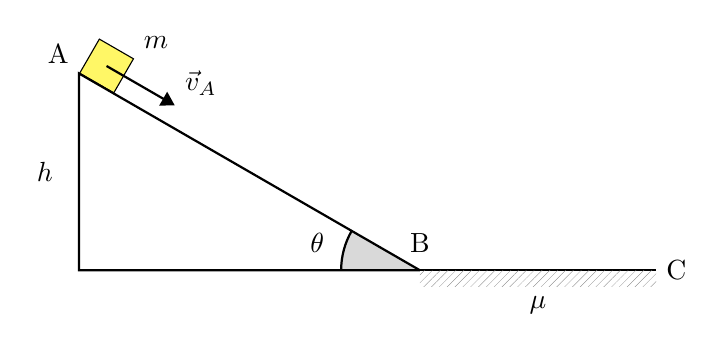
\begin{tikzpicture}[thick]

            \def\ang{150}

            % Inclined plane
            \draw (0,0) coordinate[pos=1.,label={[above=1mm]{B}}] (B)  -- ++ (\ang:5) coordinate[label=above left:A] (A) |- (B) coordinate[pos=0.5] (O);


            % Angle Theta on the background wrt the inclined plane
            \begin{scope}[on background layer]
                \pic [draw, thick, -, "$\theta$", angle eccentricity=1.35, fill=gray!30, angle radius=10mm] {angle=A--B--O};
            \end{scope}

            % Horizontal plane
            \draw   (B) -- node[below=2mm] {$\mu$} ++ (3,0) coordinate[label=right:C] (aux);
            \path   [pattern={Lines[angle=45,distance={2pt},
                  line width=0.1pt]},
                  pattern color=gray]  (B) rectangle ++ (3,-0.2);
            
        
            % h
            \draw (O) -- node[midway,left=2mm] {$h$} (A);


            % Mass
            \begin{scope}[on background layer]
                \node (M) [draw=black,
                fill=yellow!60,
                minimum width=0.5cm,
                minimum height=0.5cm,
                anchor=north east,
                rotate=\ang,
                label=south west:$m$] at (A) {};
            \end{scope}

            % Speed in A, v_A
            \draw[thick, -{Triangle[]}] (M.center) -- ++ (\ang:-1) node[above right] {$\vec{v}_A$};

 
        \end{tikzpicture}
    \end{center}
    \caption{Setting of problem \ref{prob: inclined_plane_pm_I}.}
    \label{fig: inclined_plane_pm_I}
\end{figure}
A point mass $m$ is at the top of a plane inclined by an angle $\theta$ and of height $h$. At the end of such plane there is a rough horizontal plane which has a friction of with the point mass of coefficient $\mu$. At time $t=0$ the point mass is pushed with a speed $v_A$ parallel to the inclined plane. Determine:
\begin{enumerate}[(a)]
    \item The distance travelled on the horizontal plane by the point mass before stopping;
    \item the total time of motion.
\end{enumerate}
\begin{description}
    \item[Solution 1] We can first approach this problem from a dynamic--kinematic standpoint. This means that we: i) identify all the forces acting on the point mass; ii) use Newton's second law $\mb{F} = m \mb{a}$ to determine the acceleration and thus the motion, and iii) through the equations of motion we find the quantities we need. There are only two forces acting on the point: the constraint $\mb{N}$ directed perpendicularly to the inclined plane and pointing upwards, and the weight $\mb{P}$ directed vertically downwards (\cref{fig: free_body_diagram_pm_I}). 
    \begin{figure}
        \begin{center}
            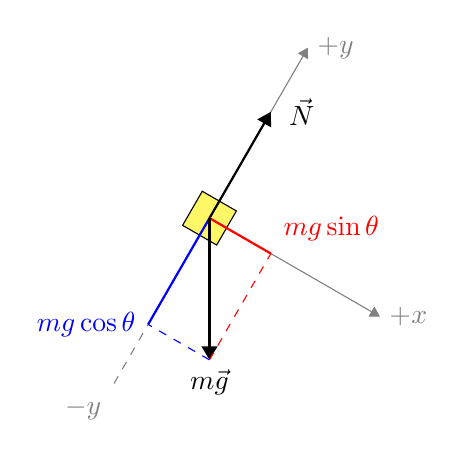
\begin{tikzpicture}[
                force/.style={draw=black,fill=black},
                axis/.style={densely dashed,gray!50,font=\small},
                M/.style={rectangle,draw,fill=yellow!60,minimum width=0.5cm,minimum height=0.5cm,},
                m/.style={rectangle,draw=black,fill=lightgray,minimum size=0.3cm,thin},
                plane/.style={draw=black,fill=blue!10},
                string/.style={draw=red, thick},
                pulley/.style={thick},
            ]
                
                \def\ang{150}
                \def\down{-90}
                \def\arcr{0.5cm}
                \def\mg{1.8}
                \def\laxis{2.5}
                %\coordinate(X) at ({\mg*sin(\ang)},0);
                %\coordinate(Y) at (0,{\mg*cos(\ang)});

                %% Free body diagram of M
                \begin{scope}[rotate=\ang-180]
                    
                    \coordinate(M) at (0,0);

                    % Mass m
                    \node[M,transform shape] (M) {};
                    
                    
                    % Draw axes and help lines
                    \draw[thin,gray=!50, -{Triangle[]}] (M.center) -- (0,\laxis) node[right] {$+y$};
                    \draw[thin,gray=!50, -{Triangle[]}] (M.center) -- ++ (\laxis,0) node[right] {$+x$};
                    \draw[thin,gray=!50,dashed] (M.center) -- ++ (0,-\laxis) node[below left] {$-y$};
                    % Indicate angle. The code is a bit awkward.

                    %\draw[solid,shorten >=0.5pt] (\down-\ang:\arcr)
                    %    arc(\down-\ang:\down:\arcr);
                    %\node at (\down-0.5*\ang:1.3*\arcr) {$\alpha$};

                    % Forces
                    % Assuming that mg = \mg. The normal force will therefore be \mg*cos(alpha)
                    \draw[thick, -{Triangle[]}] (M.center) -- ++(0,-{\mg*cos(\ang)}) node[right=1mm] {$\vec{N}$};
                    % P components
                    \draw[thick, -, red] (M.center) -- ++ ({\mg*sin(\ang)},0)  node[above right=0.3mm, red] {$mg \sin \theta$};
                    \draw[thick, -, blue] (M.center) -- ++ (0,{\mg*cos(\ang)},0)  node[left=0.3mm, blue] {$mg \cos \theta$};
                    %\draw (M.west) -- ++(-1,0) node[left] {$f_R$};
                    %\draw (M.east) -- ++(1,0) node[above] {$T$};


                \end{scope}
                % Draw P. The code is put outside the rotated
                % scope for simplicity. No need to do any angle calculations. 
                \coordinate(P) at (0,-\mg);
                \draw[thick, -{Triangle[]}] (M.center) -- ++ (P) node[below] {$m\vec{g}$};
                
                \draw[thin,blue=!50,dashed,rotate=\ang] (P) -- ++ ({\mg*sin(\ang)},0);
                \draw[thin,red=!50,dashed,rotate=\ang] (P) -- ++ (0,{\mg*cos(\ang)});


            \end{tikzpicture}
        \end{center}
        \caption{Free--body diagram for problem \ref{prob: inclined_plane_pm_I}.}
        \label{fig: free_body_diagram_pm_I}
    \end{figure}
    Let us separate the problem in two parts: the motion on the inclined plane from $A$ to $B$ and the motion on the horizontal plane from $B$ to $C$. In $AB$, let us put the $x$ axis and the $y$ axis along the inclined plane and perpendicularly to it, respectively (\cref{fig: free_body_diagram_pm_I}). Newton's law then becomes
    \begin{align}
        x: \, & P_x = m a \label{eq: acc_inclined_plane_pm_I} \\
        y: \, & N - P_y = 0,
    \end{align} 
    where the acceleration along $y$ is zero as the point only slides along the plane and not perpendicularly to it. How do we find the components of the weight? We argue that the angle between $\mb{P}$ and the negative $y$ axis is the inclination angle $\theta$: this can be seen immediately if ones realizes that the $y$ axis and $\mb{P}$ are orthogonal to the inclined plane and its base, respectively, so that the angle between these two pairs of sides have to be equal (\cref{fig: angle_P_inclined_plane}). Then
    \begin{gather}
        P_x = P \sin \theta = mg \sin \theta \label{eq: P_x_inclined_plane_pm_I} \\
        P_y = P \cos \theta = mg \cos \theta.
    \end{gather}
    Then, replacing $P_x$ from \cref{eq: P_x_inclined_plane_pm_I} into \cref{eq: acc_inclined_plane_pm_I} we get an expression for the acceleration in the tract $AB$
    \begin{equation}
        mg \sin \theta = ma_{AB} \Rightarrow a_{AB} = g \sin \theta.
    \end{equation} 
    The point acceleration is constant, thus the motion will be uniformly accelerated. The laws of motion are the following
    \begin{align}
        x(t) & = x_0 + v_0 t + \frac{1}{2} a t^2 \label{eq: x_uam} \\
        v(t) & = v_0 + at \label{eq: v_uam},
    \end{align}
    where $x_0$ and $v_0$ are the initial position and speed of the point, respectively, $a$ is the (constant) acceleration and $t$ is time.,
    What we need to find is the speed that the point has in $B$, $v_B$, as this will be the initial speed for the successive motion along the horizontal plane. We can find this quantity using the time--less formula for the uniformly accelerated motion\footnote{This formula is simply obtained by eliminating $t$ from \cref{eq: x_uam,eq: v_uam}.}
    \begin{equation}
        \label{eq: timeless_formula_uam}
        v_f^2 = v_i^2 + 2 a \Delta x,
    \end{equation}
    where $\Delta x$ is the space travelled between the initial and final time, and $a$ is constant. In our case $\Delta x = h/ \sin \theta$ is the length of the inclined plane, so that we have
    \begin{equation}
        \label{eq: speed_inclined_plane_pm_I}
        v_B = \sqrt{v_A^2 + 2 g h}.
    \end{equation}
    Now let us study the second part of the problem, that is the motion on the horizontal plane. In $BC$ the point is subject to three forces: $\mb{P}$ and $\mb{N}$ on the $y$ axis which balance themselves, and the friction $\mb{f}_a = -\mu N \hat{v}$, directed to the left along the $x$ axis. We can write
    \begin{align}
        x: \, & - \mu mg = m a_{BC} \\
        y: \, & N - P = 0,
    \end{align}
    where we have used that $N=P$ on the horizontal plane. Again the acceleration is constant in this tract
    \begin{equation}
        a_{BC} = - \mu g,
    \end{equation}
    so that we can calculate the distance inverting \cref{eq: timeless_formula_uam} for the distance travelled $\Delta x = d$
    \begin{gather}
        v_C^2 = v_B^2 + 2 a_{BC} d \Rightarrow \notag \\
        d = \frac{v_B^2}{2 \mu g} = \mybox{\frac{v_A^2}{2 \mu g} + \frac{h} {\mu}} \label{eq: d_inclined_plane_pm_I},
    \end{gather}
    where we have used that $v_C = 0$, because the problem asks for the distance travelled until the point stops, and we have taken $v_B$ from \cref{eq: speed_inclined_plane_pm_I}. Eq. \eqref{eq: d_inclined_plane_pm_I} gives us the distance travelled on the horizontal plane: if we want the \emph{total} distance we will need to add the length of the inclined plane $L = h/\sin\theta$. As for the total time of motion, we have again to add the time of the two parts, $AB$ and $BC$. 
    QED
    \item[Solution 2] Another way to go at this problem is using the formalism of mechanical energy. Specifically, we can use the law of mechanical energy conservation whenever only conservative forces are at play, and the theorem of kinetic energy where there is dissipation.

\end{description}
%%%%%%%%%%%%%%%%%%%%%%%%%%%%%%%%%%%%%%%%%%%%%%%%%%%
%%%%%%%%%%%%%%%%%%%%%%%%%%%%%%%%%%%%%%%%%%%%%%%%%%%
%%%%%%%%%%%%%%%%%%%%%%%%%%%%%%%%%%%%%%%%%%%%%%%%%%%
%%%%%%%%%%%%%%%%%%%%%%%%%%%%%%%%%%%%%%%%%%%%%%%%%%%
\section{Solid Bodies}
\subsection{Circular track and spring I}
\label{prob: circ_track_spring}
\begin{figure}
    % Circular track
    \begin{center}
        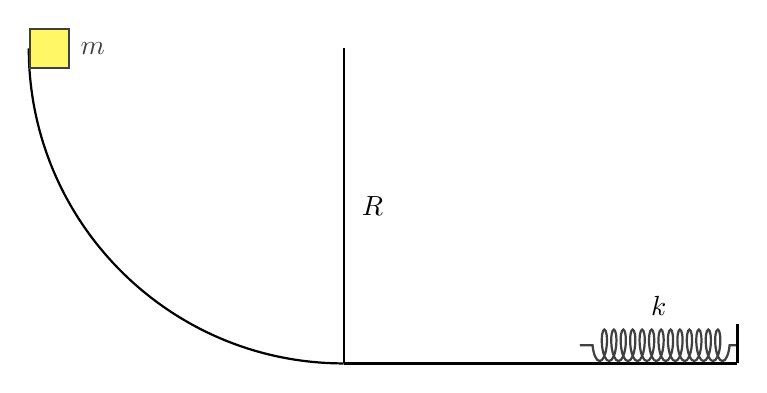
\begin{tikzpicture}[black!75,thick]
 
            % Coordinates
            \coordinate(A) at (0,0);
            \coordinate(B) at (0,4);
            \coordinate(C) at (4,4);
            \coordinate(D) at (4,0);
            \coordinate(E) at (9,0);
            \coordinate(F) at (9,0.23);
            \coordinate(G) at (7,0.23);
        
        
            % Arc
            \draw[black,thick] (B) arc[start angle=180, end angle=270, radius=4];
            \draw[black,thick] (D) -- (E);
            \draw[black,thick] (C) -- (D) node[midway,right=0.1cm,black]{$R$}; 
        
        
            % Mass
            \node[draw,
                fill=yellow!60,
                minimum width=0.5cm,
                minimum height=0.5cm,
                anchor=west,
                label=east:$m$] at (B) {};
        
        
            % Spring 
            \draw
            [
                decoration={
                    coil,
                    aspect=0.3, 
                    segment length=1.2mm, 
                    amplitude=2mm, 
                    pre length=1mm,
                    post length=1mm},
                decorate
            ] (F) -- (G) 
                node[midway,above=0.25cm,black]{$k$}; 
            \draw[black,thick] (9, 0) -- (9, 0.5);
             
        \end{tikzpicture}
    \end{center}
    \caption{Setting of problem \ref{prob: circ_track_spring}.}
    \label{fig: circular_track1}
\end{figure}

A body of mass $m$ is at the top of a circular track of radius $R$, and is left to fall at time $t=0$ with zero initial speed. At the end of the track there's a horizontal plane with a spring of stiffness $k$ at the end (\cref{fig: circular_track1}).
Determine:
\begin{enumerate}[(a)]
    \item the speed of the body when the spring is compressed by $\Delta x$, and the variation in potential energy at that point;
    \item assuming that the surface is rough and the work of the friction is $W_f < 0$, determine the maximum compression of the spring.
\end{enumerate}
\begin{description}
    \item[Solution]
    \begin{enumerate}[(a)]
        \item In the first part of the problem there is no friction and all the forces at play (gravitational and elastic) are conservative, hence we can use the conservation of mechanical energy to study the body's dynamics. Let us call $U^g = mgh$ and $U^e=\frac{1}{2}k\Delta x^2$ the gravitational and elastic potential energy, respectively. We have
        \begin{gather}
            E_i = E_f \Leftrightarrow K_i + U^g_i + U^e_i = K_f + U^g_f + U^e_f \Leftrightarrow \notag \\
            mgR = \frac{1}{2}mv_f^2 + \frac{1}{2}k\Delta x^2, \label{eq: energy_conservation1}
        \end{gather}
        where $i$ and $f$ correspond to $t=0$ and the time when the spring is compressed by $\Delta x$, respectively. $K_i=0$ since $v_i=0$, $U_i^e=0$ because the spring is not compressed at $t=0$, and $U_f^g=0$ since the height is zero on the horizontal plane. Solving \cref{eq: energy_conservation1} for $v_f$ we have
        \begin{gather}
            \frac{1}{2} m v_f^2 = mgR - \frac{1}{2}k \Delta x^2 \Rightarrow \notag \\
            \mybox{v_f = \sqrt{2gR - \frac{k}{m}\Delta x^2}}.
        \end{gather}
        QED
        \item The second part includes friction and thus a non--conservative force. As a consequence mechanical energy is not conserved, and we need to use another equation to study our problem. Specifically, we will use the kinetic energy theorem
        \begin{equation}
            \label{eq: kin_energy_th}
            W_{tot} = \Delta K,
        \end{equation}
        where $W_{tot}$ is the work generated by \emph{all} the forces acting upon the body in a given time interval $\Delta t$, and $ \Delta K $ is the variation in kinetic energy during $\Delta t$. In our case, the two time points are $t=0$, and the instant when the spring is maximally compressed which we'll call $t_m$. We then have, for the lhs and rhs
        \begin{gather*}
            W_{tot} = W_g + W_e + W_f = mgR - \frac{1}{2}k \Delta x_{max}^2 + W_f \\
            \Delta K = 0,
        \end{gather*}
        where we have used that $ W = -\Delta U $ for a conservative force. Notice that $\Delta K = 0$, because the body starts off with zero speed, and at $t_m$ the spring is maximally compressed, which also means the body has zero speed. Putting it all together we get
        \begin{equation}
            mgR - \frac{1}{2}k \Delta x_{max}^2 + W_f = 0,
        \end{equation}
        which, solving for $\Delta x$, becomes
        \begin{gather}
            \frac{1}{2}k \Delta x^2 = mgR + W_f \Rightarrow \notag \\
            \mybox{\Delta x = \sqrt{\frac{2}{k} \Bigl( mgR + W_f \Bigr)}}.
        \end{gather}
        QED
    \end{enumerate}  
\end{description}
%%%%%%%%%%%%%%%%%%%%%%%%%%%%%%%%%%%%%%%%%%%%%%%%%%%
%%%%%%%%%%%%%%%%%%%%%%%%%%%%%%%%%%%%%%%%%%%%%%%%%%%
%%%%%%%%%%%%%%%%%%%%%%%%%%%%%%%%%%%%%%%%%%%%%%%%%%%
%%%%%%%%%%%%%%%%%%%%%%%%%%%%%%%%%%%%%%%%%%%%%%%%%%%
\subsection{Inclined plane I}
\label{prob: inclined_plane_I}
A solid body of mass $m_1$ and radius $R$ is on a plane inclined by angle $\theta$. At the upper end of the solid body is attached an ideal rope, which supports a mass $m_2$. The system is initially still, the rope is tight, and the pulley is ideal. At time $t=0$, the mass $m_2$ is left free to move, and it starts to fall downward, causing the sphere to climb up the plane. The solid body's motion is of pure rolling. Determine:
\begin{enumerate}[(a)]
    \item the acceleration of mass $m_2$ and the tension of the rope $T$;
    \item the speed of the mass $m_2$ after falling by $h$.
\end{enumerate}

\begin{figure}
    \begin{center}
        \def\iangle{35} % Angle of the inclined plane
        \def\down{-90}
        \def\arcr{0.5cm} % Radius of the arc used to indicate angles
        \begin{tikzpicture}[
            force/.style={>=latex,draw=blue,fill=blue},
            axis/.style={densely dashed,gray,font=\small},
            M/.style={circle,draw,fill=yellow,minimum size=0.5cm,thin},
            m/.style={rectangle,draw=black,fill=yellow,minimum size=0.4cm,thin},
            plane/.style={draw=black,fill=gray!10},
            string/.style={draw=red, thick},
            pulley/.style={thick},
        ]
    
            
        \matrix[column sep=1cm] {
            %% Sketch
            \draw[plane] (0,-1.5) coordinate (base)
                            -- coordinate[pos=0.5] (mid) ++(\iangle:3) coordinate (top)
                            |- (base) -- cycle;
            \path (mid) node[M,rotate=\iangle,yshift=0.25cm] (M) {};
            \draw[pulley] (top) -- ++(\iangle:0.25) circle (0.3cm)
                        ++ (90-\iangle:0.5) coordinate (pulley);
            \draw[string] (M.east) -- ++(\iangle:1.5cm) arc (90+\iangle:0:0.25)
                        -- ++(0,-1) node[m] {};
    
            \draw[->] (base)++(\arcr,0) arc (0:\iangle:\arcr);
            \path (base)++(\iangle*0.5:\arcr+5pt) node {$\alpha$};
            %%
    
        &
            %% Free body diagram of M
            \begin{scope}[rotate=\iangle]
                \node[M,transform shape] (M) {};
                % Draw axes and help lines
    
                {[axis,->]
                    \draw (0,-1) -- (0,2) node[right] {$+y$};
                    \draw (M) -- ++(2,0) node[right] {$+x$};
                    % Indicate angle. The code is a bit awkward.
    
                    \draw[solid,shorten >=0.5pt] (\down-\iangle:\arcr)
                        arc(\down-\iangle:\down:\arcr);
                    \node at (\down-0.5*\iangle:1.3*\arcr) {$\alpha$};
                }
    
                % Forces
                {[force,->]
                    % Assuming that Mg = 1. The normal force will therefore be cos(alpha)
                    \draw (M.center) -- ++(0,{cos(\iangle)}) node[above right] {$N$};
                    \draw (M.west) -- ++(-1,0) node[left] {$f_R$};
                    \draw (M.east) -- ++(1,0) node[above] {$T$};
                }
    
            \end{scope}
            % Draw gravity force. The code is put outside the rotated
            % scope for simplicity. No need to do any angle calculations. 
            \draw[force,->] (M.center) -- ++(0,-1) node[below] {$Mg$};
            %%
    
        &
            %%%
            % Free body diagram of m
            \node[m] (m) {};
            \draw[axis,->] (m) -- ++(0,-2) node[left] {$+$};
            {[force,->]
                \draw (m.north) -- ++(0,1) node[above] {$T'$};
                \draw (m.south) -- ++(0,-1) node[right] {$mg$};
            }
    
        \\
        };
        \end{tikzpicture}
    \end{center}
    \caption{Setting of the problem \ref{prob: inclined_plane_I}.}
    \label{fig: inclined_plane}
\end{figure}

\begin{description}
    \item[Solution 1] 
    \begin{enumerate}[(a)]
        \item We will study the dynamics of the above system considering the cardinal equations 
        \begin{gather}
            \mb{F}_2 = m_2 \mb{a}_2 \\
            \mb{F}^{ext} = m_2 \mb{a}_{CM} \\
            \mb{M} = I_o \bm{\alpha}.
        \end{gather}  
        We then have to fix a coordinate system for each of the two bodies and find the components of the forces and the torques. Let us consider the two free--body diagrams as in \cref{fig: inclined_plane}. First let us specify what are the forces acting on the two bodies. On $m_1$ we have
        \begin{itemize}
            \item $\mb{P}_1$ acting on the center of mass downward;
            \item $\mb{T}$ acting on the upper edge towards the positive $x$--axis;
            \item $\mb{N}$ acting on the contact pointing towards the positive $y$--axis;
            \item $\mb{f}$ the friction acting on the contact point and directed along the $x$--axis -- notice that, since we are dealing with static friction, we do not know a priori what its verse is: it could be either the positive or the negative $x$--axis, and we can find this out only by solving the cardinal equations. For now we assume that $\mb{f}$ is along the negative $x$--axis.
        \end{itemize}
        On $m_2$ on the other hand we have 
        \begin{itemize}
            \item $\mb{P}_2$ directed downward;
            \item $\mb{T}$ directed upward.
        \end{itemize}
        Then for $m_2$ we can immediately write
        \begin{equation}
            P_2 - T = m_2 a_2.
        \end{equation}
        As for $m_1$, we have, along the $x$--axis
        \begin{equation}
            T - P_1 \sin \theta - f = m_1 a_{CM}.
        \end{equation}
        As for the momentum equation, let us consider the contact point as the reference to calculate all our quantities. Then $\mb{P}_1$ will have an arm equal to $R$; $\mb{T}$ has an arm $2R$, whereas $\mb{N}$ and $\mb{f}$ have zero arm and thus zero torque. Let us remember that the torque is defined as
        \begin{equation}
            \mb{M}_o = \mb{r}_o \times \mb{F},    
        \end{equation} 
        where $o$ is the reference point, and $\mb{r}$ is the arm of the force $\mb{F}$ from point $o$. Now we can immediately say that the tension $\mb{T}$ has a torque directed inwards with module $M_T = 2RT$, whereas the weight $\mb{P}_1$ has a torque directed outwards with module $P_1 R \sin (\pi - \theta)$.
        We then have
        \begin{equation}
            2RT - P_1 R \sin(\pi - \theta) = I_c \alpha,
        \end{equation}
        where $I_c$ is the moment of inertia of the solid body evaluated with respect to the contact point $C$, which we can find using the Huygens--Steiner theorem\footnote{Also called the \emph{parallel axis theorem}.}:
        \begin{equation}
            \label{eq: Ic_rolling}
            I_c = I_{CM} + m_1 R^2 = B m_1 R^2 + m_1 R^2 = (B+1) m_1 R^2 = \mathcal{B} m_1 R^2.
        \end{equation}
        In \cref{eq: Ic_rolling} we have used the fact that $I_{CM} = B m_1 R^2$, where $B$ will depend on the specific shape of the solid body. For instance, $B=1/2$ for a homogeneous cylinder, while $B=2/5$ for a homogeneous sphere. We have then called $\mathcal{B} = B+1$.
        So, putting all together we have
        \begin{equation}
            \label{eq: system_1}
            \begin{cases}
            m_1: 
            \begin{cases}
                T - P_1 \sin \theta - f = m_1 a_{CM} \\
                2RT - R P_1 \sin (\pi - \theta) = I_o \alpha
            \end{cases} \\
            m_2:
            \begin{cases}
                P_2 - T = m_2 a_2,
            \end{cases}
        \end{cases}
        \end{equation}
        which is a system of three equations with five unknowns: $T, f, a_{CM}, a, \alpha$. We then need two more equations to be able to solve the system, and we can resort to geometric relations between the accelerations. Indeed, the pure rolling of the sphere causes the point on the upper edge to have an acceleration twice as big as the center of mass'
        \begin{gather}
            a_2 = 2 a_{CM} \notag \\
            a_{CM} = \alpha R \Leftrightarrow \alpha = a_{CM}/R \notag \\
            a_{CM} = \frac{a_2}{2} \\
            \alpha = \frac{a_2}{2R}
        \end{gather}
        respectively, and these are the two further equations that we need to solve the system in \cref{eq: system_1}:
        \begin{equation}
            \label{eq: system_2}
            \begin{cases}
                T - P_1 \sin \theta - f = m_1 \frac{a_2}{2} \\
                2RT - P_1R \sin(\pi - \theta) = I_c \frac{a_2}{2R} \\
                P_2 - T = m_2 a_2.
            \end{cases}
        \end{equation}
        We can find $a_2$ by isolating $T$ from the third equation and substituting its expression in the first, to find
        \begin{equation}
            \label{eq: a_2_inclined_plane_rolling}
            a_2 = \frac{2P_2 - P_1 \sin(\pi - \theta)}{2 m_2 R + I_c/(2R)} R = \mybox{2 \frac{2m_2 - m_1 \sin\theta}{4m_2 + \mathcal{B} m_1} g}
        \end{equation}
        where we have exploited the fact that $\sin (\pi - \theta) = \sin \theta$.
        As for the tension, we can now use the third equation from the system in \cref{eq: system_2} with the expression for $a_2$ in \cref{eq: a_2_inclined_plane_rolling} to find
        \begin{gather}
            T = P_2 - m_2 a_2 = m_2 g \biggl( 1- 2 \frac{2m_2 - m_1 \sin\theta}{4m_2 + \mathcal{B} m_1} g \biggr) \notag \\
            = \mybox{\frac{m_1 m_2}{4m_2 + \mathcal{B} m_1} \Bigl( \mathcal{B} + 2 \sin \theta \Bigr) g} \label{eq: tension_inclined_plane_rolling}.
        \end{gather}
        In \cref{eq: a_2_inclined_plane_rolling,eq: tension_inclined_plane_rolling}, we can replace $\mathcal{B}$ with the corresponding values for a homogeneous cylinder or a sphere, to obtain the expressions for these two solid bodies.
        ***** insert table with values of $B$ and $\mathcal{B}$ for cylinder and sphere *******.
        QED
        \item The speed of...
    \end{enumerate}

    \item[Solution 2 - point (a) with matrices] An interesting way to solve....
\end{description}

% Thermodynamics - Problems
%\chapter{Thermodynamics}
\label{ch: thermodynamics}
\section{}

% Quantum Mechanics - Problems
\chapter{Quantum Mechanics}
\label{ch: quantum-mechanics}
\section{One Dimensional Problems}
\subsection{Harmonic oscillator and time evolution I}
The initial state of a harmonic oscillator with frequency $\omega$ and mass $m$ is given by
\begin{equation}
    \ke{ \psi (0) } = \ke{1} + i \sqrt{2} \ke{2} + (1-i) \ke{3},
\end{equation}
where $H \ke{n} = E_n \ke{n} $. Determine
\begin{enumerate}[(a)]
    \item The energy expectation value in the state $\ke{\psi (0)}$ and its standard deviation;
    \item The expectation value of the momentum operator $p$ at time $t$. 
\end{enumerate}

\begin{description}
    \item[Solution] First of all we notice a serious issue:
    \begin{equation}
        \mean{ \psi(0) | \psi(0) } = \abs{c_1}^2 + \abs{c_2}^2 + \abs{c_3}^2  = 5,
    \end{equation}
    where we have called $c_i$ the coefficient of the eigenvector $\ke{i}$. The state is not normalized and this is not acceptable since, in quantum mechanics, the square module of a state represents a probability density. In order to have a correct state $\ke{\phi (0)}$ to make our calculations we then need to normalize $\ke{\psi (0)}$, dividing it by its current module
    \begin{equation}
        \ke{\phi (0)} = \frac{1}{\sqrt{5}} \biggl( \ke{1} + i \sqrt{2} \ke{2} + (1-i) \ke{3} \biggr).
    \end{equation}
    Now we can go on make our calculations.
    \begin{enumerate}[(a)]
        \item The standard deviation of the energy is defined as 
        \begin{equation}
            \label{eq: sigma_E_harmosc}
            \sigma_E = \sqrt{\mean{E^2} - \mean{E}^2}.
        \end{equation}
        Then we need to evaluate the mean value of $E$ and $E^2$ on $\ke{ \phi (0)}$. Since our state is written in terms of eigenstates of the Hamiltonian, we can immediately calculate both
        \begin{equation}
            \mean{E}  = \frac{1}{5} \mean{ \phi (0) | H | \phi(0)} = E_1 + 2E_2 + 2E_3 = \frac{27}{10} \hbar \omega,
        \end{equation}
        where we have used that $ E_n = \hbar \omega \Bigl( n + \frac{1}{2} \Bigr)$. Similarly, we have 
        \begin{equation}
            \mean{ E^2 } = \frac{1}{5} \mean{ \phi (0) | H^2 | \phi(0)} = E_1^2 + 2E_2^2 + 2E_3^2 = \frac{157}{20} \hbar^2 \omega^2.
        \end{equation}
        Putting it all together we get
        \begin{equation}
            \label{eq: sigma_E_harmosc_number}
            \sigma_E = \sqrt{\frac{157}{20} - \frac{729}{100}} \hbar \omega = \mybox{\sqrt{\frac{14}{25}} \hbar \omega}. 
        \end{equation}
        QED
        \item $\mean{p}(t) = \mean{\phi(t) | p | \phi(t)}$. How do we obtain $\ke{\phi (t)}$? By attaching the temporal evolution to each eigenvector of the Hamiltonian 
        \begin{equation}
            \ke{\phi (t)} = \ke{1} e^{-\frac{3i \omega t}{2}} + i \sqrt{2} \ke{2} e^{-\frac{5i \omega t}{2}} + (1-i) \ke{3} e^{-\frac{7i \omega t}{2}}.
        \end{equation}
        Also, while we know the expression of the momentum operator $ p = -i \frac{d}{dx} $, we can use a more handy formula
        \begin{equation}
            \label{eq: p_ladder_harm_osc}
            p = i \sqrt{ \frac{\hbar m \omega}{2} } \bigl( a_+ - a_- \bigr),
        \end{equation}
        where $a_\pm$ are the ladder operators, that act on the eigenstates of the Hamiltonian of the harmonic oscillator as follows
        \begin{subequations}
            \label{eq: ladder_operators_harm_osc}
            \begin{align}
                a_+ \ke{n} & = \sqrt{n+1} \ke{n+1} \\
                a_- \ke{n} & = \sqrt{n} \ke{n-1}.    
            \end{align}
        \end{subequations}
        We then need to calculate the expectation values of $a_\pm$ on $\ke{\phi (t)}$, and then combine them as in Eq.~\eqref{eq: p_ladder_harm_osc} to obtain the \epv we're looking for\footnote{Note that in the second line of Eqs.~\eqref{eq: ap_phi_time},~\eqref{eq: am_phi_time} we have omitted one term in the $\ke{\cdot}$ that would have given zero upon scalar multiplication with the $\br{\cdot}$.}:
        \begin{gather}
            \mean{\phi (t) | a_+ | \phi(t)} = \frac{1}{5} \Bigl( \br{1} e^{3 i \omega t/2} - i\sqrt{2} \br{2} e^{5 i \omega t/2} + (1+i) \br{3} e^{7 i \omega t/2} \Bigr) \cdot \notag \\
            \Bigl( \sqrt{2} \ke{2} e^{-3 i \omega t/2} + i \sqrt{6} \ke{3} e^{-5 i \omega t/2} \Bigr) \cdot \notag \\
            \frac{1}{5} \Bigl( -2i e^{i \omega t} + i \sqrt{6} (1+i) e^{i \omega t} \Bigr) \label{eq: ap_phi_time},
        \end{gather}
        and, similarly
        \begin{gather}
            \mean{\phi (t) | a_- | \phi(t)} = \frac{1}{5} \Bigl( \br{1} e^{3 i \omega t/2} - i\sqrt{2} \br{2} e^{5 i \omega t/2} + (1+i) \br{3} e^{7 i \omega t/2} \Bigr) \notag \\
            \Bigl( 2 i \ke{1} e^{-5 i \omega t/2} + (1-i) \sqrt{3} \ke{2} e^{-7 i \omega t/2} \Bigr) \notag \\
            \frac{1}{5} \Bigl( 2i e^{-i \omega t} - i \sqrt{6} (1-i) e^{-i \omega t} \Bigr) \label{eq: am_phi_time}.
        \end{gather}
        Now we can put everything together
        \begin{gather}
            \mean{p}(t) = i \sqrt{\frac{\hbar m \omega}{2}} \mean{\phi(t) | a_+ - a_- | \phi(t)} = \notag \\
            \mybox{\frac{\sqrt{2 \hbar m \omega}}{5} \Bigl[ (2 - \sqrt{6}) \cos \,(\omega t) + \sqrt{6} \sin \, ( \omega t ) \Bigr]}.
        \end{gather}
        QED
    \end{enumerate}    
\end{description}
%%%%%%%%%%%%%%%%%%%%%%%%%%%%%%%%%%%%%%%%%%%%
%%%%%%%%%%%%%%%%%%%%%%%%%%%%%%%%%%%%%%%%%%%%
%%%%%%%%%%%%%%%%%%%%%%%%%%%%%%%%%%%%%%%%%%%%
%%%%%%%%%%%%%%%%%%%%%%%%%%%%%%%%%%%%%%%%%%%%
\subsection{Infinite well I}
A particle of mass $m$ is constrained in the segment $[-L/2, L/2]$. The state of the particle at time $t=0$ is 
\begin{equation}
    \psi(x) = N \cos \frac{\pi x}{L} \sin^2 \frac{2 \pi x}{L}.
\end{equation}
Determine
\begin{enumerate}
    \item The normalization constant;
    \item the \epv of the parity operator in $\psi(x)$;
    \item the possible values of an energy measurement and their relative probabilities;
    \item the probability that the particle be in $x \le 0$ as a function of time.
\end{enumerate}

\textbf{Solve}

First let us get a more handy expression of the wave--function, in terms of eigenstates of the energy. In this case we have
\begin{gather}
    E_n = \frac{2}{3}, \\
    \phi_{2k-1} = \sqrt{\frac{2}{L}} \cos \frac{(2k - 1) \pi x}{L} \\
    \phi_{2k} = \sqrt{\frac{2}{L}} \sin \frac{2k \pi x}{L},
\end{gather}
We then need to rewrite $\psi(x)$ as a linear combination of sines and cosines. Let us rewrite 
\begin{equation}
    \sin^2 t = \frac{1 - \cos 2t}{2} \Rightarrow
    \sin^2 \frac{2 \pi x}{L} = \frac{1 - \cos \frac{4 \pi x}{L}}{2}
\end{equation}
so then
\begin{gather}
    \psi (x) = \frac{N}{2} \cos \frac{\pi x}{L}\Bigl( 1 - \cos \frac{4 \pi x}{L} \Bigr) \Rightarrow \notag \\
    \psi (x) = \frac{N}{2} \Bigl[ \cos \frac{\pi x}{L} - \cos \frac{\pi x}{L} \cos \frac{4 \pi x}{L} \Bigr],
\end{gather}
but we haven't finished yet, because there's a product of cosines in the second term. We can then use Werner's formula to express it as a sum of two cosines
\begin{gather}
    \cos \alpha \cos \beta = \frac{1}{2} \Bigl[ \cos (\alpha + \beta) + \cos (\alpha - \beta) \Bigr] \notag \\
    \cos \frac{\pi x}{L} \cos \frac{4 \pi x}{L} = \frac{1}{2} \Bigl[ \cos \frac{3 \pi x}{L} + \cos \frac{5 \pi x}{L} \Bigr],
\end{gather}
and finally we have 
\begin{gather}
    \psi(x) = \frac{N}{2} \Bigl( \cos \frac{\pi x}{L} - \frac{1}{2} \cos \frac{3 \pi x}{L} - \frac{1}{2} \cos \frac{5 \pi x}{L} \Bigr) \Rightarrow \notag \\
    \psi(x) = \frac{N}{2} \sqrt{\frac{L}{2}} \bigl( \phi_1 - \frac{1}{2} \phi_3 - \frac{1}{2} \phi_5 \bigr).
\end{gather}
\begin{enumerate}
    \item At this point we can easily calculate the normalization constant $N$
    \begin{gather}
        1 = \abs{\psi (x)} = \frac{L}{2} \frac{N^2}{4} \Bigl( 1 + \frac{1}{4} + \frac{1}{4} \Bigr) = \frac{N^2 L}{8} \bigl( \frac{3}{2} \bigr) \Rightarrow \notag \\
        \mybox{N = \frac{4}{\sqrt{3 L}}}.
    \end{gather}
    QED 
    \item We can write 
    \begin{equation}
        \psi (x) = \sqrt{\frac{2}{3}} \Bigl( \phi_1 - \frac{1}{2} \phi_3 - \frac{1}{2} \phi_5 \Bigr).
    \end{equation}
    The parity operator $\hat{P}$ has the following effect on a state $\zeta(x)$
    \begin{equation}
        \hat{P} \zeta(x) = \zeta(-x),
    \end{equation}
    hence we have that
    \begin{gather}
        \mean{\hat{P}} = \int_{-L/2}^{L/2} \psi(x) \hat{P} \psi(x) dx \notag \\
        =  \int_{-L/2}^{L/2} \abs{\psi(x)}^2 dx = \mybox{1},
    \end{gather}
    where in the second line we have exploited that $\psi(-x) = \psi(x)$.
    \item The $\psi(x)$ contains the eigenfunctions of the Hamiltonian corresponding to $n \in \{ 1, 3, 5 \}$, hence the possible values of a measurement of the energy are 
    \begin{gather*}
        \mybox{E_1 = \frac{\pi^2 \hbar^2}{2 m L^2} \quad P(E_1) = \frac{2}{3}} \\
        \mybox{E_3 = \frac{9 \pi^2 \hbar^2}{2 m L^2} \quad P(E_3) = \frac{1}{6}} \\
        \mybox{E_5 = \frac{15 \pi^2 \hbar^2}{2 m L^2} \quad P(E_3) = \frac{1}{6}}. 
    \end{gather*}
    QED
    \item Let us write the state at a generic time 
    \begin{equation}
        \psi(x, t) = \sqrt{\frac{2}{3}} \Bigl( \phi_1 e^{-\frac{i E_1 t}{\hbar}} - \frac{1}{2} \phi_3 e^{-\frac{i E_3 t}{\hbar}} - \frac{1}{2} \phi_5 e^{-\frac{i E_5 t}{\hbar}} \Bigr),
    \end{equation}
    then the probability to find the electron in $[0, L/2]$ is given by (remember that $\psi(x)$, and thus its square module is even)
    \begin{gather}
        \psi(x, t) = \int_0^{L/2} \abs{ \psi(x, t) }^2 dx \notag \\
        = \frac{1}{2} \int_{-L/2}^{L/2} \abs{ \psi(x, t) }^2 dx = \mybox{\frac{1}{2}}.
    \end{gather}
    QED
\end{enumerate}
%%%%%%%%%%%%%%%%%%%%%%%%%%%%%%%%%%%%%%%%%%%%
%%%%%%%%%%%%%%%%%%%%%%%%%%%%%%%%%%%%%%%%%%%%
%%%%%%%%%%%%%%%%%%%%%%%%%%%%%%%%%%%%%%%%%%%%
%%%%%%%%%%%%%%%%%%%%%%%%%%%%%%%%%%%%%%%%%%%%
\subsection{Spin 1/2 and time evolution}
A particle of mass $m$ and spin $1/2$ has is subject to the Hamiltonian
\begin{equation}
    \label{eq: H_spin_time_evolution}
    H = 
    \begin{pmatrix}
        3 & 4 \\
        4 & -3
    \end{pmatrix}
    \hbar \omega,
\end{equation}
and, at $t=0$ is in the state
\begin{equation}
    \label{eq: psi0_time_evolution}
    | \psi (0) \rangle = \frac{1}{\sqrt{10}} ( 3 \ke{+} - \ke{-}),
\end{equation}
where $| \pm \rangle$ are the eigenstates of $S_z$ with eigenvalues $\pm \hbar/2$.
\begin{enumerate}[(a)]
    \item Find the expectation value of $S_z$ at $t=0$ and at a generic time $t$;
    \item Find the probability that a measurement of $S_z$ at time $t$ returns $\hbar/2$.
\end{enumerate}

\textbf{Solve}

\begin{enumerate}[(a)]
    \item The first question of this part is answered as follows
    \begin{equation}
        \begin{split}
            \langle S_z \rangle & = \mean{ \psi (0) | S_z | \psi (0)} = \\
            \frac{1}{10}  ( 9 & \mean{ + | S_z | +} + \mean{ - | S_z | -} ) = \\
            \frac{1}{10} & \biggl( 9 \, \frac{\hbar}{2} - \frac{\hbar}{2} \biggr) = \mybox{\frac{2}{5} \, \hbar}.
        \end{split}
    \end{equation}
    Now we need to calculate the time--dependent expectation value of $S_z$. This is achieved remembering that in the Schr\"odinger picture the time evolution lies in the state and is attached to each eigenstate of the Hamiltonian. As a consequence, a generic state at time $t$ can be written as follows
    \begin{equation}
        \ke{\psi (t)} = \sum_n \ke{\psi_n (0)} e^{-\frac{i E_n t}{\hbar}},
    \end{equation}
    where the $\psi_n$ and $E_n$ are the eigenstates and eigenvalue of the Hamiltonian operator\footnote{The Hamiltonian operator is time--independent in this picture.}. This means that we need to rewrite $\ke{\psi (0)}$ (Eq.~\eqref{eq: psi0_time_evolution}) as a linear combination of eigenvalues of $H$ (Eq.~\eqref{eq: H_spin_time_evolution}). Then we need to diagonalize the Hamiltonian:
    \begin{equation}
        \begin{split}
            \begin{vmatrix}
                3 - \lambda & 4 \\
                4 & - 3 - \lambda 
            \end{vmatrix}
            & = 0 \\
            \bigl( 3 - \lambda \bigr)  \bigl( - 3 - \lambda \bigr) & - 16 = 0,
        \end{split}
    \end{equation}
    which returns $ \lambda_{1,2} = \pm 25$. As for the eigenvectors
    \begin{equation}
        \begin{split}
            \begin{pmatrix}
                -2 & 4 \\
                4 & -8
            \end{pmatrix} &
            \begin{pmatrix}
                x \\
                y
            \end{pmatrix}
            = 0 \\
            x = 2y \Rightarrow 
            v_1 = & \frac{1}{\sqrt{5}}
            \begin{pmatrix}
                2 \\
                1
            \end{pmatrix},
        \end{split}
    \end{equation} 
    and thus 
    \begin{equation}
        v_2 = \frac{1}{\sqrt{5}}
        \begin{pmatrix}
            1 \\
            -2
        \end{pmatrix}.
    \end{equation}
    Now we have to find the expression of $\ke{ \pm }$ as linear combinations of $v_{1,2}$. Remember that $ | + \rangle = | e_1 \rangle$, $ | - \rangle = | e_2 \rangle$, the canonic base in $ \mathbb{R}^2 $. We can do it using Fourier's trick
    \begin{align}
        \ke{+} = \,  \alpha_1 & \ke{v_1} + \beta_1 \ke{v_2} \notag \\
        \alpha_1 = \mean{v_1 | +} = \frac{2}{\sqrt{5}}, & \quad \beta_1 = \mean{v_2 | +} = \frac{1}{\sqrt{5}} \notag \\
        \ke{+} = \,  \frac{1}{\sqrt{5}} ( & 2 \ke{v_1} + \beta_1 \ke{v_2} ) \label{eq: e1_spin_time_evolution}.
    \end{align}
    Analogously we find 
    \begin{equation}
        \label{eq: e2_spin_time_evolution}
        \ke{-} = \frac{1}{\sqrt{5}} \bigl( \ke{v_1} - 2 \ke{v_2} \bigr),
    \end{equation}
    and hence, replacing $\ke{\pm}$ (Eqs.~\eqref{eq: e1_spin_time_evolution} and~\eqref{eq: e2_spin_time_evolution}) in $\psi (0)$ (Eq.~\eqref{eq: psi0_time_evolution})
    \begin{equation}
        \ke{\psi (0)} = \frac{1}{\sqrt{2}} \bigl( \ke{v_1} + \ke{v_2}).
    \end{equation}
    At this point we can write the state at a generic time $t$
    \begin{equation}
        \ke{\psi (t)} = \frac{1}{\sqrt{2}}  \ke{v_1} e^{-i 5 \omega t} + \frac{1}{\sqrt{2}} \ke{v_2} e^{i 5 \omega t}.
    \end{equation}
    Since we need to find the expectation value of $\langle S_z(t) \rangle$, we have to rewrite $\psi(t)$ in terms of eigenstates of $S_z$ (this is done by inverting Eqs.~\eqref{eq: e1_spin_time_evolution},~\eqref{eq: e2_spin_time_evolution}):
    \begin{equation}
        \label{eq: psi_t_spin_1d}
        \psi(t) = \frac{1}{\sqrt{10}} ( 2 e^{-i 5 \omega t} + e^{i5 \omega t} ) | + \rangle + \frac{1}{\sqrt{10}} ( e^{-i 5 \omega t} - 2 e^{5 \omega t} ) | - \rangle.
    \end{equation}
    There we have it: we now have $\psi(t)$ expressed as a linear combination of the eigenstates of the operator whose expectation value we are interested in. Let us calculate the mean value of the Spin's $z$--component
    \begin{gather}
        \mean{ \psi (t) | \psi (t)} = \frac{\hbar}{20} \bigl( 2 e^{i 5 \omega t} + e^{-i 5 \omega t} \bigr) \bigl( 2 e^{-i 5 \omega t} + e^{i5 \omega t} \bigr) + \notag \\
        - \frac{\hbar}{20} \bigl( e^{i 5 \omega t} - 2 e^{-i 5 \omega t} \bigr) \bigl( e^{-i 5 \omega t} - 2 e^{i 5 \omega t} \bigr) = \notag \\
        \frac{\hbar}{20} \bigl[ \bigl( 5 + 2e^{i 10 \omega t} + 2e^{-i 10 \omega t} \bigr) - \bigl( 5 - 2e^{i 10 \omega t} - 2e^{-i 10 \omega t} \bigr) \bigr] = \notag \\
        \mybox{\frac{2}{5} \, \hbar \cos (10 \, \omega \, t)} \label{eq: Sexp_spin_time},
    \end{gather}
    where we have used Euler's formulas $ \cos x = \frac{e^{ix} + e^{-ix}}{2} $, $ \sin x = \frac{e^{ix} - e^{-ix}}{2} $. Eq.~\eqref{eq: Sexp_spin_time} gives us the second part of point (a). QED
    \item This point is readily answered: the square modules of the coefficients of the linear combination of $| \psi (t) \rangle$ (Eq.~\eqref{eq: psi_t_spin_1d}) return the probability to measure spin up or down. Notice that their sum adds up to one, as it is supposed to be for a correctly normalized state:
    \begin{gather}
        P(S_z = \hbar/2) = | c_+ |^2 = \frac{1}{10} \bigl( 5 + 4 \cos (10 \, \omega \, t) \bigr) = \notag \\
        \frac{1}{2} + \frac{2}{5} \cos (10 \, \omega \, t) \label{eq: P_spinup_spin_t} \\
        P(S_z = - \hbar/2) = | c_- |^2 = \frac{1}{10} \bigl( 5 - 4 \cos (10 \, \omega \, t) \bigr) = \notag \\
        \frac{1}{2} - \frac{2}{5} \cos (10 \, \omega \, t) \label{eq: P_spindown_spin_t}, 
    \end{gather}
    where we have called $c_\pm$ the coefficients of $ \ke{\pm} $ in Eq.~\eqref{eq: psi_t_spin_1d}. Eq.~\eqref{eq: P_spinup_spin_t} answers point (b) of the problem. QED 
\end{enumerate}
%%%%%%%%%%%%%%%%%%%%%%%%%%%%%%%%%%%%%%%%%%%%
%%%%%%%%%%%%%%%%%%%%%%%%%%%%%%%%%%%%%%%%%%%%
%%%%%%%%%%%%%%%%%%%%%%%%%%%%%%%%%%%%%%%%%%%%
%%%%%%%%%%%%%%%%%%%%%%%%%%%%%%%%%%%%%%%%%%%%
\section{Quantum Mechanics in Three Dimensions}
\subsection{Hydrogen atom I}
The wave--function for the hydrogen atom ground state is
\begin{equation}
    \psi_{100} = \sqrt{\frac{1}{\pi a_0^3}} e^{-r/a_0}, \qquad a_0 = \frac{4 \pi \epsilon_0 \hbar^2}{m e^2},
\end{equation}
where $a_0$ is the so--called Bohr's radius.
\begin{enumerate}[(a)]
    \item Determine the distance from the nucleus at which the probability to find the electron is maximum;
    \item Determine the mean value and standard deviation of the electron's position.
\end{enumerate}

\textbf{Solve}

The eigenstates of the hydrogen atom are given by the product of a radial function and the spherical harmonics (For a complete treatment of the hydrogen atom See~\cite{griffiths2018introduction}, Par. 4.2.)
\begin{equation}
    \label{eq: eigenstates_hydrogen_atom}
    \psi_{nlm} (r, \theta, \phi) = R_{nl} (r) Y_l^m (\theta, \phi).
\end{equation}
The quantum numbers have the following properties: $n$ is the principal quantum number and can assume all the values in $\mathbb{N}^+$; $l$ is the azimuthal quantum number $l \in \{ 0, 1, 2, \cdots n-1 \}$; $m$ is the magnetic quantum number and varies between $-l$ and $l$. Notice that every energy level has a degeneration 
\begin{equation}
    \label{eq: degeneration_h_atom}
    d(n) = \sum_{l=0}^{n-1} (2l + 1) = n^2,
\end{equation}
since to every $l$ correspond $2l+1$ values of $m$, and for every $n$ we have $n-1$ values of $l$.
The explicit expressions of the radial and spherical functions are
\begin{equation}
    R_{nl} (r) = \sqrt{\biggl( \frac{2}{n a_0} \biggr)^3 \frac{(n-l-1)!}{2n [(n+l)!]^3}} e^{-\frac{r}{n a_0}} \biggl( \frac{2r}{n a_0} \biggr)^l L_{n-l-1}^{2l+1},
\end{equation}
where 
\begin{equation}
    \label{eq: rodr_lag_gen}
    L_{p}^{q-p} (x) \equiv 1
\end{equation}
is a generalized Laguerre polynomial, and 
\begin{equation}
    \label{eq: rodr_lag}
    L_q (x) \equiv e^x \biggl( \frac{d}{dx} \biggr)^q (e^{-x} x^q)
\end{equation}
is the $q$--th Laguerre polynomial. As for the spherical harmonics, they are defined as
\begin{equation}
    Y_l^m = \epsilon \sqrt{\frac{2l + 1}{4 \pi} \frac{(l - \abs{m})!}{(l + \abs{m})!}} e^{im \phi} P_l^m (\cos \theta),
\end{equation}
where $\epsilon = (-1)^m$ for $m \ge 0$ and $\epsilon=1$ for $m<0$;
\begin{equation}
    \label{eq: rodr_leg_gen}
    P_l^m (x) \equiv ( 1 - x^2)^{\abs{m}/2} \biggl( \frac{d}{dx} \biggr)^{\abs{m}} P_l(x),
\end{equation}
is a generalized Legendre polynomial, and\footnote{Eqs.~\eqref{eq: rodr_lag_gen},~\eqref{eq: rodr_lag},~\eqref{eq: rodr_leg_gen},~\eqref{eq: rodr_leg} are called \textit{Rodrigues' formulas}.} 
\begin{equation}
    \label{eq: rodr_leg}
    P_l(x) \equiv \frac{1}{2^l l!} \biggl( \frac{d}{dx} \biggr)^l (x^2 - 1)^l
\end{equation}
is the $l$--th Legendre polynomial.

Now, we highlight that the two functions are normalized separately
\begin{gather}
    \int_0^\infty \abs{R_{nl} (r)}^2 r^2 dr = 1 \\
    \int_0^\pi \int_0^{2 \pi} \abs{Y}^2 \sin \theta d\theta d\phi = 1.
\end{gather}
That being said, let us find the answers to the problem.
\begin{enumerate}[(a)]
    \item The probability to find the electron between $r$ and $r+dr$ is given by
    \begin{equation}
        P([r, r+dr]) = \abs{\psi_{100}}^2 r^2 dr = \frac{r^2}{\pi a_0^3} e^{-\frac{2r}{a_0}}.
    \end{equation}
    The distance with maximum probability is found as follows
    \begin{gather}
        r_\textup{max} = r \, | \, \frac{d}{dr} \frac{r^2}{\pi a_0^3} e^{-\frac{2r}{a_0}} = 0 \notag \\
        \frac{2r_\textup{max}}{\pi a_0^3} \Bigl( 1 - \frac{r_\textup{max}}{a_0} \Bigr) = 0 \notag \\
        \Rightarrow \mybox{r_\textup{max}=a_0}.
    \end{gather}
    \item We need to find $\sigma_r = \sqrt{\mean{r^2} - \mean{r}^2}$. By definition, in the ground state $\psi_{100}$ we have
    \begin{gather}
        \mean{r^n} = \frac{1}{\pi a_0^3} \int_0^\infty r^{n+2} e^{-2r/a_0} dr \int_0^\pi \int_0^{2 \pi} \sin \theta d\theta d\phi = \notag \\
        4 \pi \frac{a_0^{n}}{2^{n+3} \pi} \Gamma (n+3) = 4 \pi \frac{a_0^{n}}{2^{n+3} \pi} (n+2)!,
    \end{gather}
    where $\Gamma(z)$ is the Euler's Gamma function which satisfies $\Gamma(n) = (n+1)!$ for natural $n$. Hence, we immediately find
    \begin{equation}
        \mean{r} = \mybox{\frac{3}{2} a_0}, \qquad \mean{r^2} = \mybox{3 a_0^2},
    \end{equation}
    and thus
    \begin{equation}
        \sigma_r = \sqrt{3a_0^2 - 9/4 a_0^2} = \mybox{\frac{\sqrt{3}}{2} a_0}.
    \end{equation}
    QED
\end{enumerate}
%%%%%%%%%%%%%%%%%%%%%%%%%%%%%%%%%%%%%%%%%%%%
%%%%%%%%%%%%%%%%%%%%%%%%%%%%%%%%%%%%%%%%%%%%
%%%%%%%%%%%%%%%%%%%%%%%%%%%%%%%%%%%%%%%%%%%%
%%%%%%%%%%%%%%%%%%%%%%%%%%%%%%%%%%%%%%%%%%%%
\subsection{Hydrogen atom II}
Find the state of a hydrogen atom knowing that
\begin{enumerate}[(a)]
    \item the electron is in a $p$--state with $n=2$;
    \item $P(L_z = 0) = 0$ and $\mean{L_z} = 0$;
    \item $P(0 \le \phi \le \pi/2) = 0.25$.
\end{enumerate}
The eigenstates of the hydrogen atom are given by Eq.~\eqref{eq: eigenstates_hydrogen_atom} for a generic triplet $n, l, m$. We know that $n=2$, and that the electron is in a $p$--state, hence $l=1$ and thus $ m \in \{ -1, 0, 1 \} $. 
\begin{equation}
    \psi = R_{21} (r) \bigl[ \alpha \, Y_1^1 (\theta, \phi) + \beta \, Y_1^0 (\theta, \phi) + \gamma \, Y_1^{-1} (\theta, \phi) \bigr],
\end{equation}
where $\abs{\alpha}^2 + \abs{\beta}^2 + \abs{\gamma}^2 = 1$.
However, $P(L_z) = 0 \Rightarrow \beta = 0$ and $ \mean{L_z} = 0 $, and so
\begin{equation}
    \mean{L_z} = \hbar ( \abs{\alpha}^2 - \abs{\beta}^2 ) = 0 \Rightarrow \abs{\alpha}^2 = \abs{\beta}^2 = \frac{1}{2},
\end{equation}
where the last equality follows from the normalization condition.
%%%%%%%%%%%%%%%%%%%%%%%%%%%%%%%%%%%%%%%%%%%%
%%%%%%%%%%%%%%%%%%%%%%%%%%%%%%%%%%%%%%%%%%%%
%%%%%%%%%%%%%%%%%%%%%%%%%%%%%%%%%%%%%%%%%%%%
%%%%%%%%%%%%%%%%%%%%%%%%%%%%%%%%%%%%%%%%%%%%
\subsection{}
A particle is in the following state
\begin{equation}
    \psi(x, y, z) = N e^{- \frac{x^2 + y^2 + z^2}{\sigma^2} } (x + y + z).
\end{equation}
\begin{itemize}[(a)]
    \item What are the possible values of a measurement of $\mb{L}^2$ and with what probability?
    \item What are the possible values of a measurement of $L_z$ and with what probability?
    \item Let $H = -\lambda L_z$, determine $\mean{L_z}$ and $\mean{L_x}$ as a function of time.
\end{itemize}

\textbf{Solve}

First let us write $\psi(x)$ in terms of eigenstates of $\mb{L}^2$, $L_z$. These are the spherical harmonics $Y_l^m (\theta, \phi)$, expressed in terms of spherical coordinates, which are related to the cartesian ones as follows
\begin{equation}
    \begin{cases}
        x & = r \sin \theta \cos \phi \\
        y & = r \sin \theta \sin \phi \\
        z & = r \cos \theta 
    \end{cases}
\end{equation}
so that we have 
\begin{equation}
    \psi(r, \theta, \phi) = N r e^{-\frac{r^2}{\sigma^2}} ( \sin \theta \cos \phi + \sin \theta \sin \phi  + \cos \theta).
\end{equation}
The eigenstates of the angular momentum are, for $l=1$
\begin{gather}
    Y_1^0 = \sqrt{\frac{3}{4 \pi}} \cos \theta \\
    Y_1^1 = - \sqrt{\frac{3}{8 \pi}} e^{i \phi} \cos \theta \\
    Y_1^{-1} = \sqrt{\frac{3}{8 \pi}} e^{-i \phi} \cos \theta.
\end{gather}
%%%%%%%%%%%%%%%%%%%%%%%%%%%%%%%%%%%%%%%%%%%%
%%%%%%%%%%%%%%%%%%%%%%%%%%%%%%%%%%%%%%%%%%%%
%%%%%%%%%%%%%%%%%%%%%%%%%%%%%%%%%%%%%%%%%%%%
%%%%%%%%%%%%%%%%%%%%%%%%%%%%%%%%%%%%%%%%%%%%
\subsection{Non--commuting spin components}
A particle with spin $1$ is in the state
\begin{equation}
    \ke{\psi} = \frac{1}{\sqrt{14}} 
    \begin{pmatrix}
        2 \\
        1 \\
        3i
    \end{pmatrix}.
\end{equation}
\begin{enumerate}[(a)]
    \item What is the probability that a measurement of $S_x$ yield $\hbar, 0, -\hbar$?
    \item What is the expectation value of $S_y$?
\end{enumerate}

\textbf{Solve}

We have a particle with spin one, so that the Complete Set of Commuting Operators chosen to describe the system is made of $S^2$ and $S_z$, which are expressed by the following matrices
\begin{equation}
    S^2 = 2 \hbar^2 
    \begin{pmatrix}
        1 & 0 & 0 \\
        0 & 1 & 0 \\
        0 & 0 & 1
    \end{pmatrix}, \quad
    S_z = \hbar
    \begin{pmatrix}
        1 & 0 & 0 \\
        0 & 0 & 0 \\
        0 & 0 & -1
    \end{pmatrix}.
\end{equation}
\begin{enumerate}[(a)]
    \item To calculate the probabilities to obtain a given measurement of $\langle S_x \rangle$, we need to find its matricial expression, then its eigenvectors. Once we have the eigenvectors $| v_i \rangle$, $i \in \{ 1, 2, 3 \}$ relative to the eigenvalues $ \hbar, 0, -\hbar$, we calculate the probabilities as follows
    \begin{gather}
        \label{eq: probabilities_Sx}
        P(S_x = \hbar) = | c_{1} |^2 = | \langle v_1 | \psi \rangle |^2 \\
        P(S_x = 0) = | c_{2} |^2 = | \langle v_2 | \psi \rangle |^2 \\
        P(S_x = -\hbar) = | c_{3} |^2 = | \langle v_3 | \psi \rangle |^2.
    \end{gather}  
    So how do we find the matrix $S_x$? We won't do it explicitly, but this calculation can be done considering the following equations
    \begin{subequations}
        \label{eq: Sxy_ladder}
        \begin{align}
            S_x = & \frac{S_+ + S_-}{2} \label{eq: Sx_ladder} \\
            S_y = & \frac{S_+ - S_-}{2i} \label{eq: Sy_ladder} 
    \end{align}
    \end{subequations}
    where $S_\pm$ are the ladder operators, that act on the eigenstate of $S^2$, $S_z$ as follows
    \begin{equation}
        \label{eq: S_ladder}
        S_\pm = | s, m \rangle = \hbar \sqrt{s(s+1) - m(m \pm 1)} | s, m \pm 1 \rangle.
    \end{equation}
    Using Eqs.~\eqref{eq: Sxy_ladder} and~\eqref{eq: S_ladder} we can build matrix representations of the remaining components of the spin $S_x$, $S_y$. If $S^2 = 2 \hbar^2$, we have
    \begin{equation}
        S_x = \frac{\hbar}{\sqrt{2}}
        \begin{pmatrix}
            0 & 1 & 0 \\
            1 & 0 & 1 \\
            0 & 1 & 0 
        \end{pmatrix},
    \end{equation}
    The eigenvalue equation is
    \begin{equation}
        | S_x - \lambda \mathbb{1} | = 0,
    \end{equation}
    which returns $ \lambda_{1,3} = \pm \hbar$ and $ \lambda_2 = 0$, and eigenvectors
    \begin{equation}
        \label{eq: eigenvectors_Sx}
        v_1 = \frac{1}{2}
        \begin{pmatrix}
            1 \\
            \sqrt{2} \\
            1
        \end{pmatrix}, \quad
        v_2 = \frac{1}{\sqrt{2}}
        \begin{pmatrix}
            1 \\
            0 \\
            1
        \end{pmatrix}, \quad
        v_3 = \frac{1}{2}
        \begin{pmatrix}
            1 \\
            -\sqrt{2} \\
            1
        \end{pmatrix}.
    \end{equation}
    Now, using Eq.~\eqref{eq: eigenvectors_Sx} and~\eqref{eq: probabilities_Sx} we get
    \begin{gather}
        P(S_x = \hbar) = \mybox{\frac{15 + 4 \sqrt{2}}{56}} \\
        P(S_x = \hbar) = \mybox{\frac{15 - 4 \sqrt{2}}{56}} \\
        P(S_x = \hbar) = \mybox{\frac{13}{28}},
    \end{gather}
    and this answers point (a). QED
    \item To calculate the expectation value of $S_y$ we can use Eqs.~\eqref{eq: Sy_ladder} and~\eqref{eq: S_ladder}, remembering that the eigenstates of $S^2$, $S_z$ are the canonic base $| e_i \rangle$. We then have
    \begin{gather}
        \langle S_+ \rangle = \frac{1}{14} \bigl( 2 \langle e_1 | + \langle e_2 | - 3i \langle e_3 | \bigr) \notag \\
        \hbar \sqrt{2} \bigl( | e_1 \rangle + 3i | e_2 \rangle \bigr) = \notag \\
        \frac{ \sqrt{2} \, \hbar }{14} (2 + 3i) \\
        \langle S_- \rangle = \frac{1}{14} \bigl( 2 \langle e_1 | + \langle e_2 | - 3i \langle e_3 | \bigr) \notag \\
        \hbar \sqrt{2} \bigl( 2| e_2 \rangle + | e_3 \rangle \bigr) = \notag \\
        \frac{ \sqrt{2} \, \hbar }{14} (2 - 3i) ,
    \end{gather}
    hence 
    \begin{equation}
        \label{eq: Sy_exp_Spm}
        \langle S_y \rangle = \frac{1}{2i} \langle \psi | S_+ - S_i | \psi \rangle = \mybox{\frac{3 \sqrt{2}}{14} \hbar}.
    \end{equation}
    Eq.~\eqref{eq: Sy_exp_Spm} answers point (b). QED
\end{enumerate}
%%%%%%%%%%%%%%%%%%%%%%%%%%%%%%%%%%%%%%%%%%%%
%%%%%%%%%%%%%%%%%%%%%%%%%%%%%%%%%%%%%%%%%%%%
%%%%%%%%%%%%%%%%%%%%%%%%%%%%%%%%%%%%%%%%%%%%
%%%%%%%%%%%%%%%%%%%%%%%%%%%%%%%%%%%%%%%%%%%%
\subsection{Sum of two angular momenta}
The state of a $2$--particle system is represented, in the base $ \ke{l_1, m_1}\ke{l_2, m_2}$ eigenstates of $\bm{L}_1^2, L_{1z}, \bm{L}_2^2, L_{2z}$, by the vector 
\be
    \label{eq: psi}
    \ke{\psi} = \ke{1, 1} \ke{1, -1}. 
\ee
What are the possible values of a measurement of $\bm{L}^2 $ and $L_z$ ($\bm{L} = \bm{L}_1 + \bm{L}_2$) and with what probability?
Remember that 
\be
    \label{eq: ladder_operators_Jtot}
    J_\pm \ke{l, m} = \hbar \sqrt{l(l+1) - m(m \pm 1)} \ke{l,m \pm 1}.
\ee

\textbf{Solve}

We need to write the state $\ke{\psi}$ as a linear combination of eigenstates of $\ke{l, m}$. Once done that, the square module of the coefficients of the linear combination will give us the probability to measure a given value of $\bm{L}^2, L_z$.
One simple and quick way to do it would be to use the Clebsch--Gordan tables. Upon knowing the values of $\bm{L}_1^2$ and $\bm{L}_2^2$, the Clebsch--Gordan tables contain both the coefficients necessary to write $\ke{l, m}$ as a linear combination of $ \ke{l_1, m_1}\ke{l_2, m_2}$ and vice versa. 

However, the problem does not provide us with the Clebsch--Gordan coefficients, hence this is not the way we are supposed to proceed. Another way to find the relationship between eigenstates of $\bm{L}^2, L_z$ and $\bm{L}_1^2, L_{1z}, \bm{L}_2^2, L_{2z}$ is to use the ladder operators $J_\pm$, as we will explain.

First of all, let us make a table with all the possible combination of values of $L_{1z}$ and $L_{2z}$, so as to find the possible values that $L_z$ can have.
\begin{table}
    \centering
    $\begin{array}{c@{\hspace{1.5cm}}c@{\hspace{1.5cm}}c}
        \toprule
        L_{1z} & L_{2z} & L_z \\
        \midrule
        -1 & -1 & -2 \\
        -1 & 0 & -1 \\
        -1 & 1 & 0 \\
        \midrule
        0 & -1 & -1 \\
        0 & 0 & 0 \\
        0 & 1 & 1 \\
        \midrule
        1 & -1 & 0 \\
        1 & 0 & 1 \\
        1 & 1 & 2 \\
        \bottomrule
    \end{array}$   
    \caption{Table with all the possible values of $L_{1z}, L_{2z}$ and $L_z$.}   
    \label{tab: Lz_tot_11} 
\end{table}
The problem tells us that we have two particles with $l_1 = l_2 = 1$. As we see can from table~\ref{tab: Lz_tot_11}, in this case the possible values for $m$ range from $-2$ to $2$. In particular, we have nine possible values, through which we can reconstruct: i) the five states for $l=2; m \in \{-2, -1, 0, 1, 2 \}$; ii) the triplet $l=1; m \in \{-1, 0, 1 \}$ and iii) the singlet $l=0; m=0$.
At this point we know the possible eigenstates of the total angular momentum $\ke{l, m}$ once we have two particles with $l_1 = l_2 = 1$. Now we need to find out how to write our state $\ke{\psi}$ in terms of $\ke{2, m}, \ke{1, m}$ and $\ke{0, 0}$. So how do we go about to do that? The idea is the following. We know that each state $\ke{l, m}$ will be a linear combination of specific eigenstates of $\bm{L}_1^2, L_{1z}, \bm{L}_2^2, L_{2z}$, that we can find using the table~\ref{tab: Lz_tot_11}. For instance, we know that a state with $m=1$ can only be obtained adding $m_1=0, m_2=1$ or $m_1=1, m_2=0$ (rows six and eight):
\begin{align}
    \label{eq: L1_states}
    \ke{2, 1} & = \alpha \ke{1, 1}_1 \ke{1, 0}_2 + \beta \ke{1, 0}_1 \ke{1, 1}_2 \\
    \ke{1, 1} & = \delta \ke{1, 1}_1 \ke{1, 0}_2 + \gamma \ke{1, 0}_1 \ke{1, 1}_2.     
\end{align}
The problem is that we do not know the coefficients $\alpha, \beta, \gamma, \delta$, and similarly we do not know the coefficients for writing most of the states $\ke{l, m}$. However, looking at table~\ref{tab: Lz_tot_11} we notice that there are some states that are obtained only with a single combination of $m_1, m_2$:
\begin{align}
    \ke{2, 2} & = \ke{1, 1}_1 \ke{1, 1}_2 \label{eq: L2m2_states_1} \\
    \ke{2, -2} & = \ke{1, -1}_1 \ke{1, -1}_2 \label{eq: L2m2_states_2}.
\end{align}
Eqs.~\eqref{eq: L2m2_states_1},\eqref{eq: L2m2_states_2} come to our rescue, as they allow us to have a starting point to use to obtain all the other states $\ke{l, m}$. How? By applying the ladder operators $J_\pm$ (Eq.~\eqref{eq: ladder_operators_Jtot}), that have the effect of lowering the $m$ when applied on $\ke{l, m}$. But the $J_\pm$ act on eigenstates of $\bm{L}^2, L_z$, so how do we obtain the expression of these states in terms of eigenstates of $\bm{L}_1^2, L_{1z}, \bm{L}_2^2, L_{2z}$? Simply by remembering that
\be
    \label{eq: JpmLpm}
    J_\pm = L_{1\pm} + L_{2\pm},
\ee
where $L_{1\pm}, L_{2\pm}$ behave just as $J_\pm$ (Eq.~\eqref{eq: ladder_operators_Jtot}) but on $\ke{l_1, m_1}, \ke{l_2, m_2}$, respectively
\be
    \label{eq: ladder_operators_L}
    L_{i \pm} = \ke{l_i, m_i} = \hbar \sqrt{l_i(l_i+1) - m_i(m_i \pm 1)} \ke{l_i,m_i \pm 1}.
\ee

There we have it: we start from Eq.~\eqref{eq: L2m2_states_1}, then we apply the ladder operators $J_\pm$ on the left-hand side (Eq.~\eqref{eq: ladder_operators_Jtot}), and $L_{i \pm}$ on the rhs (Eq.~\eqref{eq: ladder_operators_L}), and we can build all the states for a given value $l$. And what about states with other values of $l$, for instance, $\ke{1, 1}$? For these, we observe that the two states in Eqs.~\eqref{eq: L2m2_states_1},~\eqref{eq: L2m2_states_1} are orthogonal, since the set of eigenvalues of a hermitian operator are an orthonormal basis of the vector space the operator acts on -- hence we would have, for instance,
\be
    \label{eq: orthog_L21L11}
    \mean{2, 1 | 1, 1} = 0.
\ee
Eq.~\eqref{eq: orthog_L21L11} allows us to find the expression of all the remaining states\footnote{We can assume that the relative phases are all zero.}.

Let's go and solve this problem then. First of all, we notice that we start from a state where $m_1 = 1, m_2 = -1$, which gives $m=0$ (see table~\ref{tab: Lz_tot_11}), and thus we have that
\be
    \label{eq: psi_J}
    \ke{\psi} = a \ke{2, 0} + b \ke{1, 0} + c \ke{0, 0}.
\ee
Eq.~\eqref{eq: psi_J} tells us that the only possible value for a measurement of $L_z$ is zero, with probability $P(L_z=0) = 1$, and this answers one part of the question. We still need to determine the probabilities to obtain different values of $\bm{L}^2$.

We start from Eq.~\eqref{eq: L2m2_states_1}, $\ke{2, 2} = \ke{1, 1}_1 \ke{1, 1}_2$. Applying the ladder operators on both sides we get:
\be
    J_{-} \ke{2, 2} = 2 \hbar  \ke{2, 1}
\ee
on the lhs, and 
\be
    (L_{1-} + L_{2-} ) \ke{1, 1} \ke{1, 1} = \hbar \sqrt{2} \bigl( \ke{1, 0} \ke{1, 1} + \ke{1, 1} \ke{1, 0} \bigr) 
\ee
on the rhs. Putting it all together we find
\be
    \ke{2, 1} = \frac{1}{\sqrt{2}} \bigl( \ke{1, 0} \ke{1, 1} + \ke{1, 1} \ke{1, 0} \bigr).
\ee
Exploiting the condition in Eq.~\eqref{eq: orthog_L21L11} we immediately find another state
\be
    \ke{1, 1} = \frac{1}{\sqrt{2}} \bigl( \ke{1, 0} \ke{1, 1} - \ke{1, 1} \ke{1, 0} \bigr).
\ee
Now we need to obtain the states with zero $L_z$, so we apply once more the ladder operators to $\ke{2, 1}$:
\be
    \label{eq: J20_lhs}
    J_{-} \ke{2, 1} =  \hbar \sqrt{6} \ke{2, 0} 
\ee
and
\begin{equation}
    \begin{split}
        \label{eq: J20_rhs}
        (L_{1-} + L_{2-} ) & \bigl( \ke{1, 0} \ke{1, 1} + \ke{1, 1} \ke{1, 0} \bigr) = \\ \hbar \sqrt{2} & \bigl( \ke{1, -1} \ke{1, 1} + 2 \ke{1, 0} \ke{1, 0} + \ke{1, 1} \ke{1, -1} \bigr), 
    \end{split}
\end{equation}
and thus 
\be
    \label{eq: J20}
    \ke{2, 0} = \frac{1}{\sqrt{6}} \bigl( \ke{1, -1} \ke{1, 1} + 2 \ke{1, 0} \ke{1, 0} + \ke{1, 1} \ke{1, -1} \bigr)
\ee
Doing the same with $\ke{ 1, 0 }$ we find
\be
    \label{eq: J10}
    \ke{1, 0} = \frac{1}{\sqrt{6}} \bigl( \ke{1, -1} \ke{1, 1} - \ke{1, 1} \ke{1, -1} \bigr).
\ee
Finally, we need $\ke{0, 0}$, which we can find noticing that
\be
    \label{eq: J00_cl}
    \ke{0, 0} = a_1 \ke{1, -1} \ke{1, 1} + b_1 \ke{1, 0} \ke{1, 0} + c_1 \ke{1, 1} \ke{1, -1}
\ee
and that $\bk{ 2, 0 }{ 0, 0 } = \bk{ 1, 0 }{ 0, 0 } = 0$. Doing so returns
\be
    \label{eq: J00}
    \ke{0, 0} = \frac{1}{\sqrt{3}} \bigl( \ke{1, -1} \ke{1, 1} - \ke{1, 0} \ke{1, 0} + \ke{1, 1} \ke{1, -1} \bigl).
\ee
At this point we have all the states that we are interested in, that is $\ke{2, 0}$, $\ke{1, 0}$, $\ke{0, 0}$ in terms of $\ke{l_1, m_1} \ke{l_2, m_2}$. Using Eq.~\eqref{eq: psi_J} and Eqs.~\eqref{eq: J00},~\eqref{eq: J10},~\eqref{eq: J20} we can find the coefficients of the linear combination using Fourier's trick
\begin{align}
    a & = \bigl( \br{1, 1} \br{1, -1}  \bigr) \ke{2, 0} = \frac{1}{\sqrt{6}} \\
    d & = \bigl( \br{1, 1} \br{1, -1}  \bigr) \ke{1, 0} = \frac{1}{\sqrt{2}} \\
    c & = \bigl( \br{1, 1} \br{1, -1}  \bigr) \ke{0, 0} = \frac{1}{\sqrt{3}}.
\end{align}
Hence, we finally can write
\be
    \label{eq: psi_J_eigenstates}
    \ke{\psi} = \frac{1}{\sqrt{6}} \ke{2, 0} + \frac{1}{\sqrt{2}} \ke{1, 0} + \frac{1}{\sqrt{3}} \ke{0, 0}.
\ee
At this point the problem is solved. In fact, Eq.~\eqref{eq: psi_J_eigenstates} tells us that a measurement of $\bm{L}^2$ can return\footnote{Remember that the eigenvalue of $\bm{L}^2$ is $l(l+1) \hbar^2$.} i) $6 \hbar^2$ with probability $P(\bm{L}^2 = 6 \hbar^2) = 1/6$; ii) $2 \hbar^2$ with probability $P(\bm{L}^2 = 2 \hbar^2) = 1/2$ and iii) $0$ with probability $P(\bm{L}^2 = 0) = 1/3$. QED
%%%%%%%%%%%%%%%%%%%%%%%%%%%%%%%%%%%%%%%%%%%%
%%%%%%%%%%%%%%%%%%%%%%%%%%%%%%%%%%%%%%%%%%%%
%%%%%%%%%%%%%%%%%%%%%%%%%%%%%%%%%%%%%%%%%%%%
%%%%%%%%%%%%%%%%%%%%%%%%%%%%%%%%%%%%%%%%%%%%
\section{Perturbation Theory}
\subsection{Perturbation to infinite well}
A particle of mass $m$ is in a one--dimensional infinite potential well in $[0, L]$. Calculate the first--order perturbative corrections to the ground state and the first excited state due to the following perturbation
\be
    \label{eq: perturbation}
    H' = \epsilon E_0 \frac{x}{L}
\ee
where $E_0$ is the unperturbed ground--state energy.

\textbf{Solve}

The particle is subject to the following Hamiltonian
\be
    \label{eq: h_particle}
    H = H_0 + H',
\ee
where $H_0$ is the unperturbed Hamiltonian
\be
    H_0 = \frac{p^2}{2 m} + V(x),
\ee
with
\be
V(x)=
\begin{cases}
0 & \text{if $x \in [0, L]$} \\
\infty & \text{otherwise}
\end{cases}
\ee
The unperturbed problem is a well--known one for which we know the full solution, that is, eigenstates and eigenvalues of the Hamiltonian operator (see~\cite{griffiths2018introduction}, Par. 2.2):
\begin{align}
    E_n^{(0)} & = \frac{n^2 \pi^2 \hbar^2}{2 m L^2} \quad n \in \mathbb{N}^+ \label{eq: En_inf_well } \\
    \psi_n^{(0)}(x) & = \sqrt{\frac{2}{L}} \sin \biggl( \frac{n \pi}{L} x \biggr) \label{eq: psin_inf_well},
\end{align}
which we will call the solutions to order zero, hence the subscript. How do we find the first--order perturbative corrections? The answer depends on whether the energy level we consider is degenerate. In our case, there are no degenerate levels, hence the energy corrections to the first order are given by the following formula (see~\cite{griffiths2018introduction}, Par. 6.1)
\be
    \label{eq: E1_pert_nondeg}
    E_n^{(1)} = \mean{ \psi_n^{(0)} | H' | \psi_n^{(0)}}.
\ee
In our case, Eq.~\eqref{eq: E1_pert_nondeg} becomes
\begin{equation}
    E_n^{(1)} = \frac{\epsilon E_0}{L} \mean{\psi_n^{(0)} | x | \psi_n^{(0)}} = \frac{\epsilon E_0}{L} \langle x \rangle_n^{(0)}.
\end{equation}
Now, the expectation value of $x$ is always in the middle of the well, regardless of the energy level\footnote{To see this, move the well to $[-L/2, L/2]$. Then the potential is even, and the eigenstates of $H$ will be either even or odd. As a consequence, $\langle \psi_n^{(0)} | x | \psi_n^{(0)} \rangle$ = 0.}, $\langle x \rangle_n^{(0)} = L/2$. The proof is simple:
\begin{equation}
    \begin{split}
        \langle x \rangle_n^{(0)} & = \frac{2}{L} \int_0^L x \sin^2 \biggl( \frac{n \pi}{L} x
        \biggr) \, dx = \\
        & \frac{2L}{n^2 \pi^2} \int_0^{n\pi} y \sin^2 y \, dy,
    \end{split}
\end{equation}
where we made the substitution $y = n \pi x/L$. Now we isolate the integral and integrate it by parts, writing $\sin y = - (\cos y)'$
\begin{equation}
    \begin{split}
        \int_0^{n\pi} y \sin^2 y \, dy & = -y \sin y \cos y \bigg|_0^{n\pi} + \int_0^{n\pi} \cos y (\sin y + y \cos y) \, dy = \\
        & \int_0^{n\pi} \frac{\sin 2y}{2} + \int_0^{n\pi} y - \int_0^{n\pi} \sin^2 y \, dy,
    \end{split}
\end{equation}
where the first contour term is zero, and we have used that $\sin 2y = 2 \sin y \cos y$, and $\cos^y = 1 - \sin^2 y$. Finally, moving the last integral to the lhs, we find
\begin{equation}
    \int_0^{n\pi} y \sin^2 y \, dy = \frac{1}{2} \int_0^{n\pi} y = 
    \frac{y^2}{4} \biggl|_0^{n\pi} = \frac{n^2 \pi^2}{4},
\end{equation}
hence 
\begin{equation}
    \langle x \rangle_n^{(0)} = \frac{2 L}{n^2 \pi^2} \frac{n^2 \pi^2}{4} = \frac{L}{2}.
\end{equation}
Putting it all together, we have
\begin{equation}
    \label{eq: 1st_order_corr_inf_well}
    E_n^{(0)} = \frac{\epsilon E_0}{L} \langle x \rangle_n^{(0)} = \frac{\epsilon E_0}{2}.
\end{equation}
There we have it: the first--order correction to the $n$--th state is given by Eq.~\eqref{eq: 1st_order_corr_inf_well}. QED
%%%%%%%%%%%%%%%%%%%%%%%%%%%%%%%%%%%%%%%%%%%%
%%%%%%%%%%%%%%%%%%%%%%%%%%%%%%%%%%%%%%%%%%%%
%%%%%%%%%%%%%%%%%%%%%%%%%%%%%%%%%%%%%%%%%%%%
%%%%%%%%%%%%%%%%%%%%%%%%%%%%%%%%%%%%%%%%%%%%
\subsection{}
Consider the Hamiltonian $H = H_0 + H'$, with
\begin{equation}
    H_0 = 
    \begin{pmatrix}
        \frac{\hbar \omega}{2} & 0 & 0 \\
        0 & \frac{3 \hbar \omega}{2} & 0 \\
        0 & 0 & \frac{5 \hbar \omega}{2} 
    \end{pmatrix}
    \quad \quad \quad
    H' = 
    \begin{pmatrix}
        0 & ia & 0 \\
        -ia & 0 & 0 \\
        0 & 0 & 0
    \end{pmatrix},
\end{equation}
with $a \in \mathbb{R}$. Find the energy corrections to the first non--null perturbative level. Discuss the energy shifts and compare these to the exact result assuming $ a \ll \hbar \omega$.

\textbf{Solve}

First we notice that $H'$ is Hermitian, that is $(H')^{\dag} = H'$. This is a necessary condition for an observable operator, as it ensures that its eigenvalues are real. That being said, the problem is solvable analytically, diagonalizing the matrix sum $H$
\begin{equation}
    H =
    \begin{pmatrix}
        \frac{\hbar \omega}{2} & ia & 0 \\
        -ia & \frac{3 \hbar \omega}{2} & 0 \\
        0 & 0 & \frac{5 \hbar \omega}{2} 
    \end{pmatrix}.
\end{equation}
We then need to solve the equation
\begin{equation}
    \left| H - \lambda \mathbb{I} \right| = 0 \quad \Longleftrightarrow \quad
    \begin{vmatrix}
        \frac{\hbar \omega}{2} - \lambda & ia & 0 \\
        -ia & \frac{3 \hbar \omega}{2} - \lambda & 0 \\
        0 & 0 & \frac{5 \hbar \omega}{2} - \lambda
    \end{vmatrix} = 0,
\end{equation}
that becomes
\begin{gather}
        \biggl( \frac{5 \hbar \omega}{2} - \lambda \biggr) \biggl[  \biggl( \frac{\hbar \omega}{2} - \lambda \biggr) \biggl( \frac{3 \hbar \omega}{2} - \lambda \biggr) - a^2 \biggr] = 0 \notag \\
        \biggl( \frac{5 \hbar \omega}{2} - \lambda \biggr) \bigl( 4 \lambda^2 - 8 \hbar \omega \lambda + 3 \hbar^2 \omega^2 - 4 a^2 \bigr) = 0,
\end{gather}
hence the three eigenvalues, that is, the three exact energies are
\begin{equation}
    \label{eq: exact_energies}
    E_1^e = \hbar \omega - \frac{1}{2} \sqrt{\hbar^2 \omega^2 + 4 a^2} \qquad
    E_2^e = \hbar \omega + \frac{1}{2} \sqrt{\hbar^2 \omega^2 + 4 a^2} \qquad
    E_3^e = \frac{5 \hbar \omega}{2} 
\end{equation}
The eigenvectors are normalized vectors that solve the three systems
\begin{equation}
    \begin{pmatrix}
        \frac{\hbar \omega}{2} - \lambda_i & ia & 0 \\
        -ia & \frac{3 \hbar \omega}{2} - \lambda_i & 0 \\
        0 & 0 & \frac{5 \hbar \omega}{2} - \lambda_i
    \end{pmatrix}
    \begin{pmatrix}
        x \\
        y \\
        z
    \end{pmatrix} 
    \quad i \in \{ 1, 2, 3 \},
\end{equation}
but we won't find them here because we don't need to.
Let us now turn to solving the perturbation problem. The correction to first order are found using the equation $E_n^{(1)} = \langle \psi_n^{(0)} | H' | \psi_n^{(0)} \rangle$, where the $|\psi_n^{(0)} \rangle = \ke{e_n}$, that is the canonic base in $\mathbb{R}^3$. Looking at $H'$, we can see that the $E_n^{(1)} = 0$ for every $n$. Hence, the perturbative corrections to first order are zero for every state. We thus need to resort to the second--order perturbative corrections, which are given by the equation (see~\cite{griffiths2018introduction}, Par. 6.1)
\begin{equation}
    \label{eq: E2_pert_nondeg}
    E_n^{(2)} = \sum_{m \ne n} \frac{| \langle \psi_m^{(0)} | H' | \psi_n^{(0)} \rangle |^2 } {E_n^{(0)} - E_m^{(0)}}.
\end{equation}
Now, we call $H_{mn}' = \langle \psi_m^{(0)} | H' | \psi_n^{(0)} \rangle |$. Because $H'$ is hermitian, we know that $H_{mn}' = (H_{nm}')^*$, and thus $ \left| H_{mn} \right|^2 = \left| H_{nm} \right|^2 $. The corrections are
\begin{align}
    \label{eq: En_2order}
    E_1^{(2)} & = \frac{\left| H_{21} \right|^2}{E_1^{(0)} - E_2^{(0)}} + \frac{\left| H_{31} \right|^2}{E_1^{(0)} - E_3^{(0)}} \\
    E_2^{(2)} & = \frac{\left| H_{12} \right|^2}{E_2^{(0)} - E_1^{(0)}} + \frac{\left| H_{32} \right|^2}{E_2^{(0)} - E_3^{(0)}} \\
    E_3^{(2)} & = \frac{\left| H_{13} \right|^2}{E_3^{(0)} - E_1^{(0)}} + \frac{\left| H_{23} \right|^2}{E_3^{(0)} - E_2^{(0)}},  
\end{align}
we then need to calculate $ H_{12} $, $ H_{13} $, $ H_{23} $. Let us start with $H_{12} = \langle e_1 | H' | e_2 \rangle$
\begin{equation}
    \label{eq: H12}
    \begin{split}
        H_{12} = \bigl( 1 \quad 0 \quad 0 \bigr)
        \begin{pmatrix}
            0 & ia & 0 \\
            -ia & 0 & 0 \\
            0 & 0 & 0
        \end{pmatrix} &
        \begin{pmatrix}
            0 \\ 
            1 \\
            0
        \end{pmatrix} = \\
        \bigl( 1 \quad 0 \quad 0 \bigr) &
        \begin{pmatrix}
            0 \\ 
            1 \\
            0
        \end{pmatrix} = ia,
    \end{split}
\end{equation}
Following a similar calculation we find that $H_{13} = 0$ and $H_{23} = 0$. Using these results in~\eqref{eq: En_2order} we obtain the second--order corrections to all the energy levels
\begin{align}
    E_1^{(2)} & = -\frac{a^2}{\hbar \omega} \\
    E_1^{(2)} & = \frac{a^2}{\hbar \omega} \\
    E_3^{(2)} & = 0.
\end{align}
Finally, the energies to second order are
\begin{align}
    \label{eq: En_2order_complete}
    \mathcal{E}_1^{(2)} & = \frac{\hbar \omega}{2} - \frac{a^2}{\hbar \omega} \\
    \mathcal{E}_2^{(2)} & = \frac{3 \hbar \omega}{2} + \frac{a^2}{\hbar \omega} \\
    \mathcal{E}_3^{(2)} & = \frac{5 \hbar \omega}{2}.
\end{align}
So, the perturbation to second order show that the ground level shifts to a lower energy state, while the energy of the first excited state slightly increases. Lastly, the second excited state remains untouched: this is due to the fact that the perturbation matrix has no elements on the $3^\textup{rd}$ row\footnote{Since the perturbation matrix has to be hermitian, having no elements on row $i$ translates into having no elements on column $i$.}.

Let us now compare these results with the exact results in Eq.~\eqref{eq: exact_energies} in the limit $a \ll \hbar \omega$. In said case we can expand $E_1^e$ and $E_2^e$ ($E_3^e$ has no corrections) about $ a/(\hbar \omega) \simeq 0$
\begin{equation}
    \label{eq: E12_exact}
    E_{1,2}^e = \hbar \omega \mp \frac{1}{2} \hbar \omega f(x),
\end{equation}
where we have put $ f(x) = \sqrt{1 - 4 x^2}$ and $x= a/(\hbar \omega)$. We then need to expand $f(x)$ about zero
\begin{equation}
    \begin{split}
        f(x) & \simeq f(0) + f'(0) x + \frac{1}{2} f''(0) x^2 \\
        f(x) & \simeq 1 + \frac{4 x}{\sqrt{1 + 4 x^2}} \biggl|_{x=0}  + \frac{1}{2} \frac{4}{(1 + 4x^2)^{3/2}} \biggl|_{x=0} x^2 \\
        f(x) & \simeq 1 + 2x^2,
    \end{split}
\end{equation}
which, together with Eq.~\eqref{eq: E12_exact}, gives
\begin{align}
    E_{1}^e & \simeq \frac{\hbar \omega}{2} - \frac{a^2}{\hbar \omega} \\
    E_{2}^e & \simeq \frac{3 \hbar \omega}{2} + \frac{a^2}{\hbar \omega}.
\end{align}
So there we have it, the second--order approximation to the exact energies. These coincide with the second--order perturbative corrections (Eq.~\eqref{eq: En_2order_complete}): this is expected, since the $n$--th order perturbative corrections are obtained by expanding the exact eigenvalue equation (see~\cite{griffiths2018introduction} Par. 6.1). QED
%%%%%%%%%%%%%%%%%%%%%%%%%%%%%%%%%%%%%%%%%%%%
%%%%%%%%%%%%%%%%%%%%%%%%%%%%%%%%%%%%%%%%%%%%
%%%%%%%%%%%%%%%%%%%%%%%%%%%%%%%%%%%%%%%%%%%%
%%%%%%%%%%%%%%%%%%%%%%%%%%%%%%%%%%%%%%%%%%%%
\subsection{Harmonic oscillator perturbation I}
Consider a one--dimensional harmonic oscillator electrically charged in a constant electric field.
\begin{enumerate}[(a)]
    \item Calculate the energy corrections to first and second perturbative order, and the first--order correction to the eigenstates;
    \item in this case the problem can be solved exactly. Find the exact energies and verify that they are consistent with the perturbative corrections.
\end{enumerate}

\textbf{Solve}

First let us determine the explicit expression of the Hamiltonian
\begin{equation}
    H = H_0 + H' = \frac{p^2}{2 m} + \frac{1}{2} k x^2 + H',
\end{equation}
where $H'$ is the electric potential energy due to a constant electric field
\begin{equation}
    \label{eq: H_pert_const_E}
    H' = U_e = - L = - \int_0^x q \mathcal{E} dx' = -q \mathcal{E} x.
\end{equation}
We then have 
\begin{equation}
    \label{eq: harm_osc_linear_pert}
    H = \frac{p^2}{2 m} + \frac{1}{2} k x^2 - q \mathcal{E} x.
\end{equation}
\begin{enumerate}[(a)]
    \item The first--order perturbative corrections are given by Eq.~\eqref{eq: E1_pert_nondeg}. In our case it becomes 
    \begin{equation}
        E_n^{(0)} = -q \mathcal{E} \mean{n \, | x \, | \, n},
    \end{equation}
    where $H_0 \ke{n} = E_n \ke{n}$. We notice that $x$ can be written in terms of the ladder operators~\eqref{eq: ladder_operators_harm_osc} as 
    \begin{equation}
        \label{eq: x_ladder_harm_osc}
        x = \sqrt{\frac{\hbar}{2 m \omega}} (a_+ + a_-).
    \end{equation}
    Since $a_+$ and $a_-$ raise and lower the energy state respectively, we have that the corrections to first order are zero for every energy level
    \begin{equation}
        E_n^{(1)} = 0.
    \end{equation}
    As for the first--order corrections to the eigenstates, they are given by the formula (see~\cite{griffiths2018introduction}, Par. 6.1)
    \begin{equation}
        \label{eq: first_order_pert_psi}
        \psi_n^{(1)} = \sum_{m \ne n} \frac{\mean{\psi_m^{(0)} \, | \, H' \, | \, \psi_n^{(0)}}}{E_n^{(0)} - E_m^{(0)}} \psi_m^{(0)}.
    \end{equation}
    Notice that~\eqref{eq: first_order_pert_psi} applies when the $n$--th energy level is non--degenerate, otherwise a different formula is needed (see~\cite{bransden1989introduction}, Par. ). In our case the corrections to first order are then
    \begin{equation}
        \psi_n^{(1)} = - \frac{q \mathcal{E}}{\omega} \sqrt{\frac{1}{2 m \hbar \omega}} ( \sqrt{n}\psi_{n-1}^{(0)} - \sqrt{n+1} \psi_{n+1}^{(0)} ),
    \end{equation}
    so that every state $\psi_n^{(0)}$ gets a first--order correction that includes its successive and previous states with slightly different coefficients. 

    We then have to calculate the corrections to second order, that are given by Eq.~\eqref{eq: E2_pert_nondeg}. The only terms that are not zero are the ones with $m = n+1$ and $m=n-1$
    \begin{gather}
        E_n^{(2)} = \frac{ \abs{(H')_{n-1,n}^2} }{\hbar \omega} - \frac{ \abs{(H')_{n+1,n}^2} }{\hbar \omega} = \notag \\
        \frac{q^2 E^2}{2 m \omega^2} (n + 1 - n) = \frac{q^2 E^2}{2 m \omega^2}.
    \end{gather}
    \item The problem in Eq.~\eqref{eq: harm_osc_linear_pert} is exactly solvable using a simple trick:
    \begin{gather}
        H = \frac{p^2}{2 m} + \frac{1}{2} m \omega^2 x^2 - q \mathcal{E} x = \notag \\
        \frac{p^2}{2 m} + \frac{1}{2} m \omega^2 ( x - x_0 )^2 - \frac{1}{2} m \omega^2 x_0^2,
    \end{gather}
    where we have added and subtracted $ x_0^2 = \frac{q^2 \mathcal{E}^2}{m \omega^2} $ to form the square. Now, upon replacing
    \begin{equation}
        \label{eq: sub_harm_linear_pert}
        y = x - x_0,
    \end{equation}
    we recover the Hamiltonian of the harmonic oscillator plus a constant 
    \begin{equation}
        \label{eq: ham_harm_linear_pert}
        H(y, p) = \frac{p^2}{2 m} + \frac{1}{2} m \omega^2 y^2 - \frac{q^2 \mathcal{E}^2}{2 m \omega^2},
    \end{equation}
    so that the energy levels are shifted 
    \begin{equation}
        H(y, p) \ke{n} = \biggl( E_n^{(h)} - \frac{q^2 \mathcal{E}^2}{2 m \omega^2} \biggr) \ke{n} = E_n \ke{n},
    \end{equation}
    where $ E_n^{(h)} $ are the energy levels of the simple harmonic oscillator
    \begin{equation}
        \label{eq: En_harm_osc}
        E_n^{(h)} = \hbar \omega \Bigl( n + \frac{1}{2} \Bigr).
    \end{equation}
    So then 
    \begin{equation}
        \mybox{E_n = \hbar \omega \Bigl( n + \frac{1}{2} \Bigr) - \frac{q^2 \mathcal{E}^2}{2 m \omega^2}}.
    \end{equation}
    What about the eigenstates? The eigenfunctions of the harmonic oscillator are given by (see~\cite{griffiths2018introduction}, Par. 2.3)
    \begin{equation}
        \psi_n^{(h)}(x) = \biggl( \frac{m \omega}{\pi \hbar} \biggr)^{1/4} \frac{1}{\sqrt{2^n \, n!}} \, H_n \biggl( \sqrt{\frac{m \omega}{\hbar}} x \biggr) e^{- \frac{m \omega}{2 \hbar} x^2},
    \end{equation}
    where 
    \begin{equation}
        \label{eq: rodr_herm}
        H_n (x) = (-1)^n e^{x^2} \Bigl( \frac{d}{dx} \Bigr)^n e^{-x^2}
    \end{equation}
    are the Hermite polynomials. The Hermite polynomials remain the eigenfunctions of the Hamiltonian~\eqref{eq: ham_harm_linear_pert}, but with the substitution in Eq.~\eqref{eq: sub_harm_linear_pert},
    \begin{gather}
        \psi_n(x) = \psi_n^{(h)}(x-x_0) = \notag \\ 
        \mybox{\biggl( \frac{m \omega}{\pi \hbar} \biggr)^{1/4} \frac{1}{\sqrt{2^n \, n!}} \, H_n \biggl( \sqrt{\frac{m \omega}{\hbar}} ( x - x_0 ) \biggr) e^{- \frac{m \omega}{2 \hbar} (x - x_0)^2}}.
    \end{gather}
    QED
\end{enumerate}
%%%%%%%%%%%%%%%%%%%%%%%%%%%%%%%%%%%%%%%%%%%%
%%%%%%%%%%%%%%%%%%%%%%%%%%%%%%%%%%%%%%%%%%%%
%%%%%%%%%%%%%%%%%%%%%%%%%%%%%%%%%%%%%%%%%%%%
%%%%%%%%%%%%%%%%%%%%%%%%%%%%%%%%%%%%%%%%%%%%
\section{Linear Algebra}
\subsection{Commuting operators}
\begin{enumerate}[(a)]
    \item Prove that, if two matrices commute in a given base, then they commute in any base
    \begin{equation}
        \label{eq: commutator_change_base}
        [ \mb{T}_1^e, \mb{T}_2^e ] = \mathbf{0} \Rightarrow [ \mb{T}_1^f, \mb{T}_2^f ] = \mathbf{0}.
    \end{equation}
    \item Show that two matrices that are simultaneously diagonalizable commute.
\end{enumerate}

\textbf{Solve}

Let us consider a base $\ke{e_i}$, $i \in \{1, \cdots, n \}$ in a given vector space $\mathcal{V}$. If we change the base to a new one $\ke{f_i}$, we can expres the old base vectors as linear combinations of the new ones
\begin{gather}
    \ke{e_1} = S_{11} \ke{f_1} + S_{21} \ke{f_2} + \cdots + S_{n1} \ke{f_n}, \notag \\
    \ke{e_2} = S_{12} \ke{f_1} + S_{22} \ke{f_2} + \cdots + S_{n2} \ke{f_n}, \notag \\
    \cdots \notag \\
    \ke{e_n} = S_{1n} \ke{f_1} + S_{2n} \ke{f_2} + \cdots + S_{nn} \ke{f_n},
\end{gather}
that is, in short,
\begin{equation}
    \label{eq: old_base_new_base}
    \ke{e_j} = \sum_{i=1}^n S_{ij} \ke{f_i}, \quad j \in \{ 1, 2, \cdots , n \}.
\end{equation}
So how does a vector transform upon said change of base? If 
\begin{equation}
    \ke{a} = \sum_j a_j^e \ke{e_j}
\end{equation}
in the old base, then in the new base 
\begin{gather}
    \ke{a} = \sum_{i,j} a_j^{e} S_{ij} \ke{f_j} = \notag \\
    \sum_j \sum_i S_{ij} a_j^{e} \ke{f_j},
\end{gather}
so that the coefficients in the new base are
\begin{equation}
    a_j^f = \sum_i S_{ij} a_j^e.
\end{equation}
In matricial form 
\begin{equation}
    \label{eq: a_change_base}
    \mathbf{a}^f = \mathbf{Sa}^e.
\end{equation}
Let us now consider a matrix $\mathbf{T}^e$ representing a linear transformation in the old base $ \ke{e_i} $; how does it change upon switching to a new base? In the old base we had
\begin{equation}
    \mathbf{b}^e = \mathbf{T}^e \mathbf{a}^e.
\end{equation}
Let us multiply Eq.~\eqref{eq: a_change_base} to the left by\footnote{Notice that $\mb{S}^{-1}$ exists, otherwise the new vectors $\ke{f_i}$ would not cover the entire vector space, and thus would not be a base.} $ \mathbf{S}^{-1} $ so as to obtain $ \mathbf{a}^e = \mathbf{S}^{-1} \mathbf{a}^f $. Then we can write
\begin{gather}
    \mathbf{b}^f = \mathbf{S} \mathbf{b}^e = \mathbf{S} \mathbf{T}^e \mathbf{a}^e = \\
    \mathbf{S} \mathbf{T}^e \mathbf{S}^{-1} \mathbf{a}^f.
\end{gather}
We then have that the matrix $\mb{T}$ transforms as 
\begin{equation}
    \label{eq: T_change_base}
    \mb{T}^f = \mathbf{S} \mathbf{T}^e \mathbf{S}^{-1}.
\end{equation}
\begin{enumerate}[(a)]
    \item At this point we can use Eq.~\eqref{eq: T_change_base} to prove Eq. \eqref{eq: commutator_change_base}:
    \begin{gather}
        [ \mb{T}_1^f, \mb{T}_2^f ] = \mb{T}_1^f \mb{T}_2^f - \mb{T}_2^f \mb{T}_1^f = \notag \\
        \mb{S} \mb{T}_1^e \mb{S}^{-1} \mb{S} \mb{T}_2^e \mb{S}^{-1} - \mb{S} \mb{T}_2^e \mb{S}^{-1} \mb{S} \mb{T}_1^e \mb{S}^{-1} = \notag \\
        \mybox{\mb{S} [ \mb{T}_1^e, \mb{T}_2^e] \mb{S}^{-1} = \mb{0}}.
    \end{gather}
    QED
    \item from point (a) we know that if two matrices commute in one base, they also commute in any other base. Let us then consider the base where the two $n \text{x} n$ matrices of are diagonalized
    \begin{equation}
        \mb{A} = 
        \begin{pmatrix}
            \alpha_1 &  &  &  \\
             & \alpha_2 &  &  \\
             & & \ddots & \\
             &  &  & \alpha_n
        \end{pmatrix},
        \qquad
        \mb{B} = 
        \begin{pmatrix}
            \beta_1 &  &  &  \\
             & \beta_2 &  &  \\
             & & \ddots & \\
             &  &  & \beta_n
        \end{pmatrix}
    \end{equation}
    so that the products are both
    \begin{equation}
        \mb{AB} = \mb{BA} =
        \begin{pmatrix}
            \alpha_1 \beta_1 &  &  &  \\
             & \alpha_2 \beta_2 &  &  \\
             & & \ddots & \\
             &  &  & \alpha_n \beta_n
        \end{pmatrix} 
    \end{equation}
    and thus 
    \begin{equation}
        \mybox{[ \mb{A}, \mb{B} ] = \mathbf{0}}.
    \end{equation}
    QED
\end{enumerate}




%~


\backmatter

\clearpage
\bibliography{notes} 
\bibliographystyle{plain}

\end{document}
~








\section{THINGS TO DO}






